
\documentclass{article}

\usepackage[UTF8]{ctex}


\usepackage{graphicx}
\usepackage{hyperref}
\usepackage{amsmath}
\usepackage{algorithm}
%\usepackage{algorithmic}
\usepackage{algpseudocode}
\usepackage{subcaption}
\usepackage{booktabs}


\usepackage[
  paper  = letterpaper,
  left   = 1.25in,
  right  = 1.25in,
  top    = 1.0in,
  bottom = 1.0in,
  ]{geometry}
\usepackage{setspace}

% For importing python source code, from https://tex.stackexchange.com/questions/83882/how-to-highlight-python-syntax-in-latex-listings-lstinputlistings-command

\usepackage{color}
\definecolor{deepblue}{rgb}{0,0,0.5}
\definecolor{deepred}{rgb}{0.6,0,0}
\definecolor{deepgreen}{rgb}{0,0.5,0}

% Default fixed font does not support bold face
\DeclareFixedFont{\ttb}{T1}{txtt}{bx}{n}{12} % for bold
\DeclareFixedFont{\ttm}{T1}{txtt}{m}{n}{12}  % for normal
\DeclareFixedFont{\ttfuck}{T1}{txtt}{m}{n}{12}  % for normal


\usepackage{listings}

% Python style for highlighting
\newcommand\pythonstyle{\lstset{
language=Python,
basicstyle=\ttm,
otherkeywords={self},             % Add keywords here
keywordstyle=\ttb\color{deepblue},
emph={MyClass,__init__},          % Custom highlighting
emphstyle=\ttb\color{deepred},    % Custom highlighting style
stringstyle=\color{deepgreen},
frame=tb,                         % Any extra options here
showstringspaces=false,             
breaklines=true,                 % come from https://tex.stackexchange.com/questions/243500/python-code-block-outside-of-margin
}}


% Python environment
\lstnewenvironment{python}[1][]
{
\pythonstyle
\lstset{#1}
}
{}

% Python for external files
\newcommand\pythonexternal[2][]{{
\pythonstyle
\lstinputlisting[#1]{#2}}}

% Python for inline
\newcommand\pythoninline[1]{{\pythonstyle\lstinline!#1!}}



\graphicspath{{images/}}

\title{使用贝叶斯推断方法探测隐藏敌人单位探测}

\author{卓越羿 
\footnote{LaTeX代码(英/中文)和实验文件已经托管在GitHub,见: 
\url{ https://github.com/yiyuezhuo/Undergraduate-thesis } 。原文以英语写成,受制于学校规定翻译成了中文}
}

\date{2018}

\begin{document}

\maketitle

\begin{abstract}

Assuming a location which have samller distance to two conflict factions have higher probability causing a battle,
how do we infer the location of enemy if we can only observe the locations of allies and battles? 
The latent variable inference problem requieres a suitable front probability model and a effiecent way to run the 
inference. In this work, a battle model is introduced and a bayes inference framework based on pytorch 
is developed to reach the inference task including point, movement detection and 
exist probability estimation with different prior and various initialization value setting.
A case study about The battle of Gettysburg is included to show the overview of the content covered by the paper.

假设一个位置离敌我双方单位越近,则有更高的爆发一场战斗的概率。应当如何推断敌方单位的位置如果我们
只能观测到友方和战斗发生的位置?这种隐变量推断问题需要一个设定恰当的正向生成概率模型一个有效的算法
借此进行反向推断。本文提出几个战役模型以及编写了一个基于pytorch的贝叶斯推断框架,将它们应用到
点和运动探测,存在概率估计上,分别使用了均匀先验和其他数据相关的先验。它们也都使用了不同
的初始值测试算法的有效性。文章最后包含一个葛底斯堡战役的案例研究覆盖全文讨论的内容。

\end{abstract}

\tableofcontents



\section{介绍}

In real warfare, you can't observe enemy units even allies units as RTS or classic board wargame way.
The only thing you can rely on are complex and confusing even self-contradiction information and misinformation.
There're a lot of example, that general misunderstand information and may be defeated due to this. 
Bing Sun manipulated field kitchen of his army to trick his opponent, General McClellan reject to attack
due to "peace gun"(fake gun instrument) seted by south rebels, lossing oppotunity to beat rebel down.

Unfortunately, current military decision similation program, 
such as "classic" wargame (a example see Figure~\ref{fig:hps}) and somewhat  "serious" RTS, 
tend to capture more "macro" aspect and simplify the reconnaissance and 
information modeling aspect into a unaccepted level.

在真实战场上,你不能观测到像RTS和经典桌上兵棋那样直接观测到敌方单位,甚至连友方单位都不能观测到。
你能依赖的唯一的东西就是那些混乱复杂乃至自相矛盾的信息和谣言。有很多因为错误信息导致失败的例子,
如孙膑减灶愚弄对手,麦克莱伦将军因为南方军设的“和平炮”
\footnote{下文将经常提到美国内战的例子,特别是葛底斯堡战役作为案例研究,
这是因为作者曾长时间推演HPS内战/拿破仑系列兵棋。对此比较了解}(装扮成炮的道具)而驻兵不前,
从而失去一举击败邦联的机会。

不幸的是,当前军事决策模拟程序,如经典兵棋(一个例子可见图~\ref{fig:hps})和某些“严肃”RTS,
总是试图去捕捉更“宏大”的层面(倒也许和他们荒谬的宏大叙事历史学同行不同),而对侦查和信息使用
这类难以难以建模又不有趣的东西避之不及,乃至采用了过度的简化。

\begin{figure}[ht]
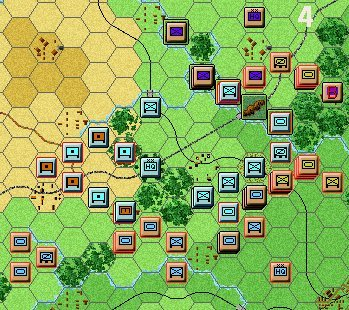
\includegraphics[width=0.6\linewidth]{SmolenskR4.jpg}
\caption{This figure show the reconnassance treatment of Smolensk' 41, 
a classic hex wargame developed by HPS.
Units can only be observed wholly or can't be observed.
图中展示了经典兵棋公司HPS的作品斯摩棱斯克41对侦查的处理——单位仅能出于完全可知和完全不可知的状态。 }
\label{fig:hps}
\end{figure}

Though we can read the oob(order of battle) as Figure~\ref{fig:metz} from map of battle, 
but it's obvious that those marks are placed in there using post Liang Zhuge information. 
In real time battle field, you can only hear where be attacked and where observe the trace of enemy 
(instead of unit detail id or somewhat weird strange quatity information), 
and some of them may be wrong and some of them may be released by enemy to confuse you.
The movement of Jackson in valley campaign is a vivid example about how the fake information intentionally
made by oppnent get the change to weaken the strength of army.

尽管我们经常可以直接在事后画的战场局势图上看到战斗序列(即那些方框图标),如图~\ref{fig:metz}。
但是显然这些标记是根据事后对照双方信息才得以制成的,在真实战场上,我们并不能指望某些“地图模拟软件”
一样如此看到敌人踪迹,甚至还包括明显不应该能观测到的量化信息。真的传到达的很可能是错的或者误导信息。
杰克逊将军在谷地利用迷惑性行动使得林肯政府和指挥手足无措就是个生动的例子。


\begin{figure}[ht]
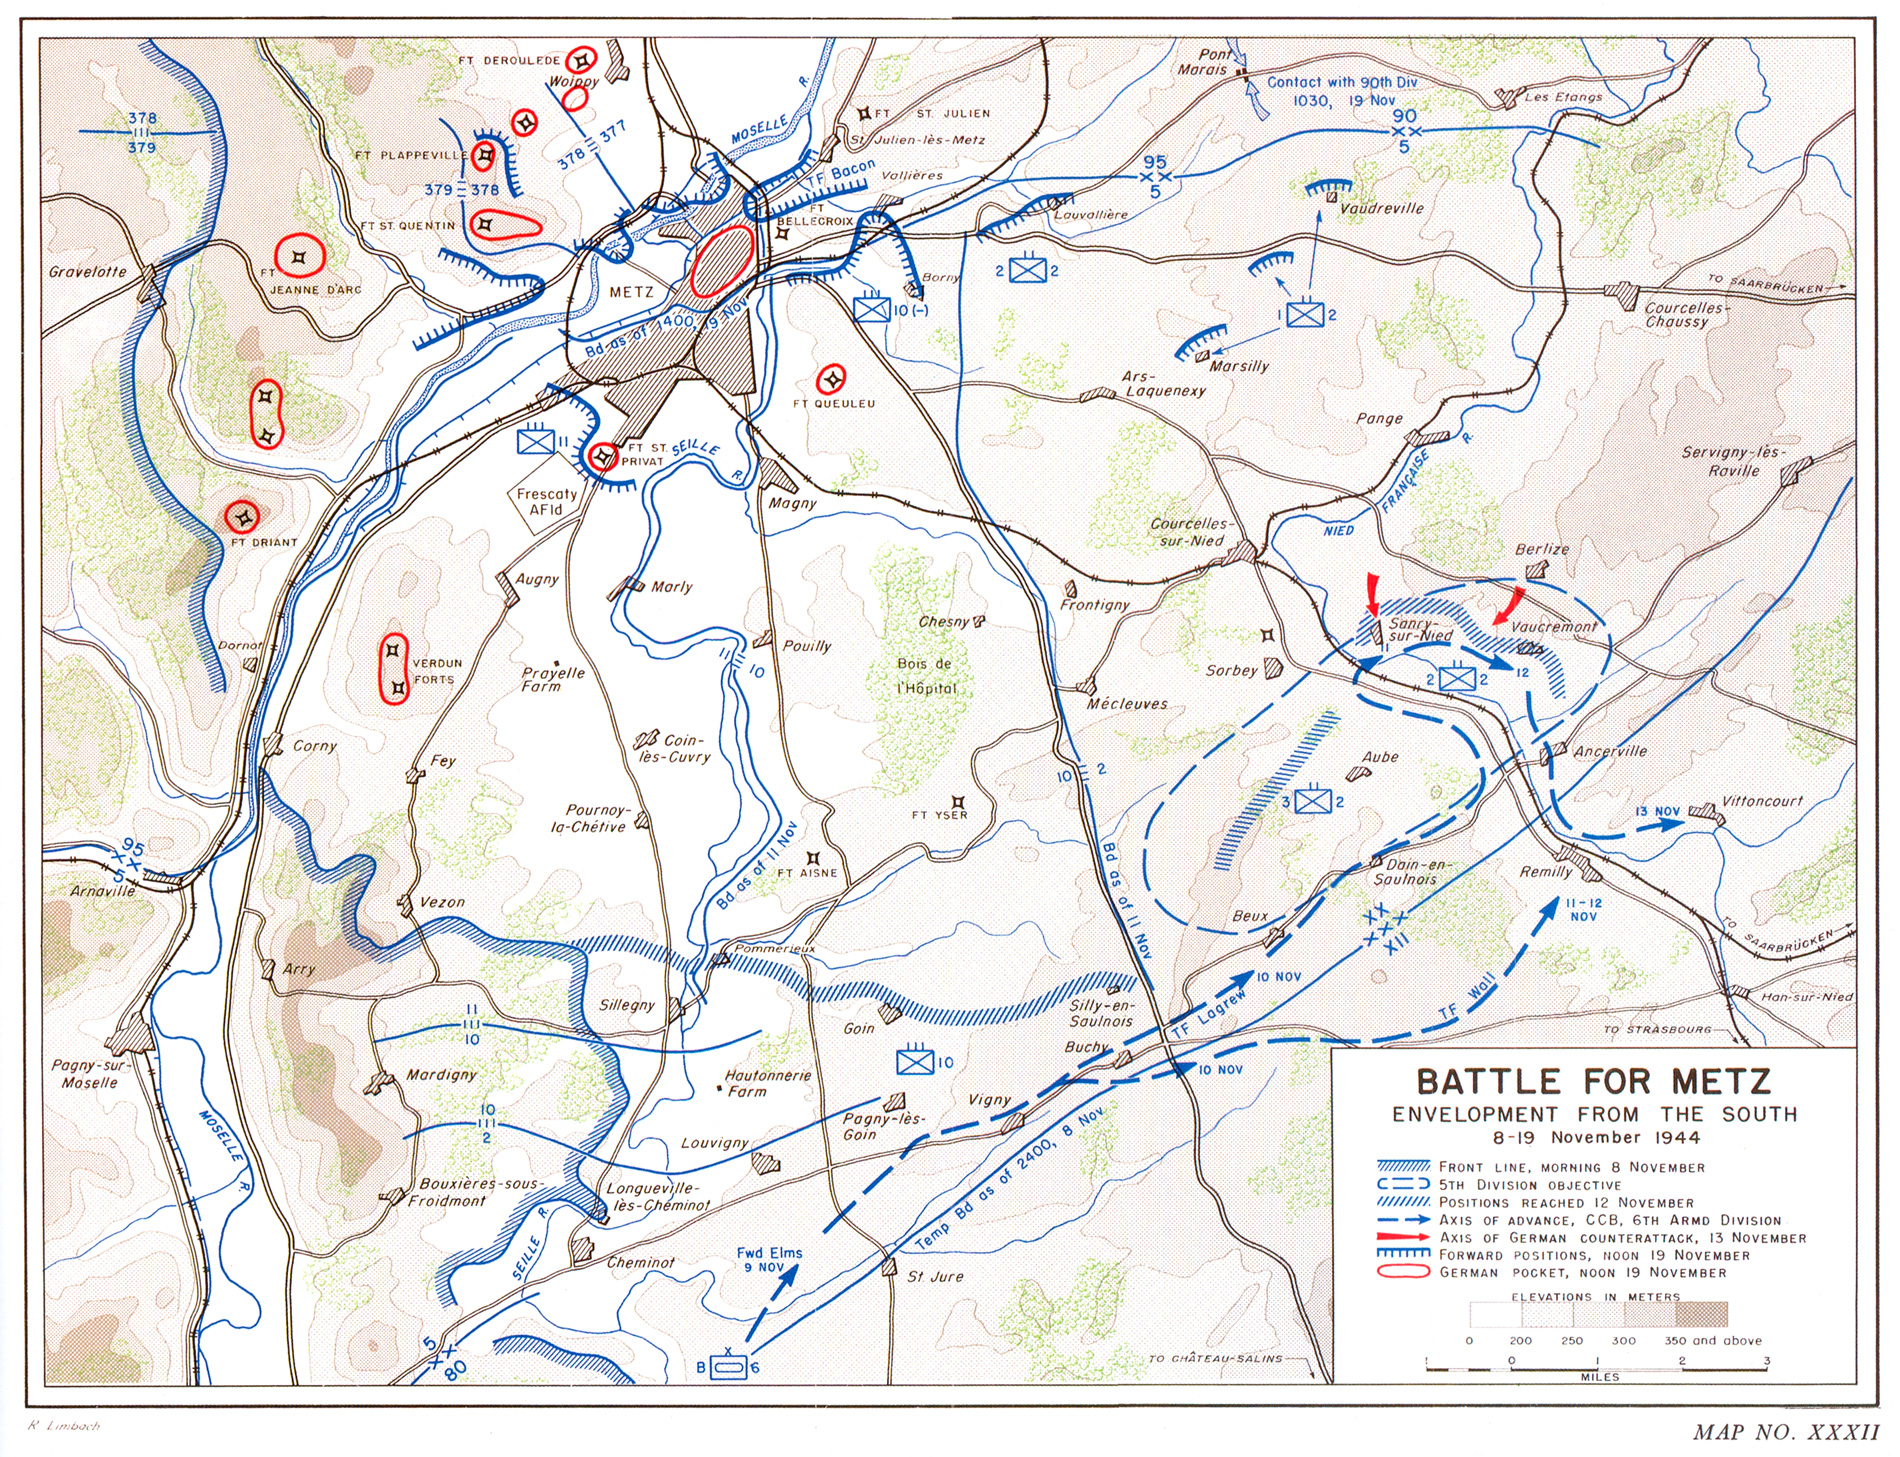
\includegraphics[width=0.6\linewidth]{metz.jpg}
\caption{The map of battle of Metz, showing oob that can't be observed in real time battlefied.
梅兹战役地图,地图展示了并不应该在真实战场上所能看到的OOB }
\label{fig:metz}
\end{figure}


There are some work were made to solve this problem 
\cite{hostetler2012inferring} \cite{vsmejkal2016integrating} \cite{touhou}.
Since they filter small part of information from replay file, they made a case that enemy can not be 
seen in that direct way, then they proposed according probability model to rebuild real situation.
Those're good tries, but not real demands for most of case. The paper we
\footnote{Though the paper only have a writer, 
but "we" seems a traditional and kind pronoun for such paper. 
In following content, both "we" and "I" will be used to represent the writer.} 
wrote will deal the problem in a more direct and intuitive way. 
A coordinate based position and movement detecting method is present in this paper.

已经有一些工作致力于解决这一信息处理方式过于简单暴力的问题,如
\cite{hostetler2012inferring} \cite{vsmejkal2016integrating} \cite{touhou}。
这些工作手动将完全信息中的一大部分屏蔽,虽然这种屏蔽类似特征工程所做的,但目的并非使得算法更有效,
而是手动模拟出一个信息不完全环境来测试一些处理算法。不过总的来说它们并不是很有用。本文将以
一种更直接,直觉的方式解决这个问题,主要围绕位置和运动的探测展开。

\section{构建恰当正向生成模型}

\subsection{简单模型}

In forward model, a process that can give probility of number of battles and the mass in support space 
is required. For example, given ally and ememy location setting as Figure~\ref{fig:stateNoBattle}.

在正向生成模型中,可以定义一个二维随机点过程,首先抽一个战役数量,然后独立同分布的从一个二维分布中
抽取那个数量的战役坐标。例如,给定如图~\ref{fig:stateNoBattle}所示友军和敌军的地点位置:

\begin{figure}[ht]
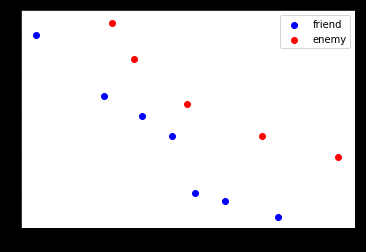
\includegraphics{state_no_battle.png}
\caption{Ally and enemy setting
友军和敌军的位置设定}
\label{fig:stateNoBattle}
\end{figure}


Suppose the the number of battle is $10$ 
\footnote{ Though the number can modeled as it draw from a given distribution by adding 
stochastic process, it be not adpoted due to its extra difficulty in express.}
, we can model the $10$ battles are indepently drawn from below distribution:

假定战役数是$10$\footnote{为了简化,后文的战役数都是给定的而不是随机过程的一部分。}
于是可设这$10$个战役是从下述分布所抽取出来的:

$$
P(x,y) \propto \max_i p^A_{i}(x,y) \max_j p^E_{j} (x,y)
$$

Where $p^A_{i}(x,y)$ indicate the probability density "released" from of i’st ally unit,
$p^E_{j}$ indicate same thing from j’st enemy unit. And the density is defined by:

这里 $p^A_{i}(x,y)$ 表示第$i$个友方单位“散布”出来的概率密度,
$p^E_{j}$ 表示第$j$个敌方单位单位对应的密度。这个密度又被定义为:


$$
P^S_i(x,y) \propto \exp(-\frac{1}{2}((x-x^S_i)^2 + (y-y^S_i)^2))
$$

Where the probability in $(x,y)$ released from i'th unit of S side($S \in \{A,E \}$). 
So the above formula can be rewritten as: 

表示$S$方($S \in \{A,E  \}$)第$i$个单位在点$(x,y)$释放的概率。故而上式可被重写为: 

$$
P(x,y) \propto \exp(-\frac{1}{2}((x-x_{nearst(x,y)})^2 + (y-y_{nearst(x,y)})^2))
$$

Where $nearst(x,y)$ point to the unit(enemy or ally) which is nearest to (x,y).

This means the non-normalized probability is only subject to the nearest two conflict units’s distance. 
Though the assumption don’t have abundant meaning,
it capture something crucial but have obvious weakness such as independent hypothesis, 
lately the model will be adujusted mutiple times to resolve this and other problems. 
Anyway, the probability can be computed and visualized as contour Figure~\ref{fig:stateNoBattleProb}.

这里$nearst(x,y)$表示离点$(x,y)$最近的单位(敌方或友方)。

这么定义使得此非标准化概率仅仅被决定于两个最近的冲突单位的距离。这个来自两个单位在以其为位置为中心的
区域内漫游而碰撞的自然推导,不过它们是独立的抽出来等假设显然是不对的。之后这个模型会被修改和比较。

无论如何,现在标准化概率可以被计算出来并如等高线图~\ref{fig:stateNoBattleProb}所示。

\begin{figure}[ht]
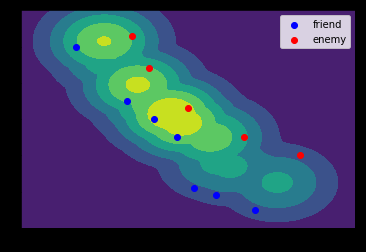
\includegraphics{state_no_battle_prob.png}
\caption{Battle density distribution 战役发生概率密度分布}
\label{fig:stateNoBattleProb}
\end{figure}

The probability distribution don't have a standard shape, implying it's hard to sample. 
To overcome this, the "grid sampling" technology is used. In this example,
 the support of density is limited to $[-1,5] \times [0,6]$
(that is, the point out of set $[-1,5] \times [0,6]$ have zero density). 
And $100 \times 100$ points are selected to build a grid approxmation. 
See a size-reduced example serve to eye in Figure~\ref{fig:gridify}.

显然这个概率分布的形状并不是哪种已知解析形式,从而从它中采样变成了个难题。 
这里使用所谓格采样法解决这个问题,考虑到这个问题的维度并不高。本例中,首先限制
密度的非零区域只取在 $[-1,5] \times [0,6]$上。
然后等距取$100 \times 100$个点作为对应小区域之密度的近似,
然后转为一个此区域所具有的离散概率所对应的随机变量。
一个采样率更小粒度更大的示意图可见于图~\ref{fig:gridify}。


\begin{figure}[ht]
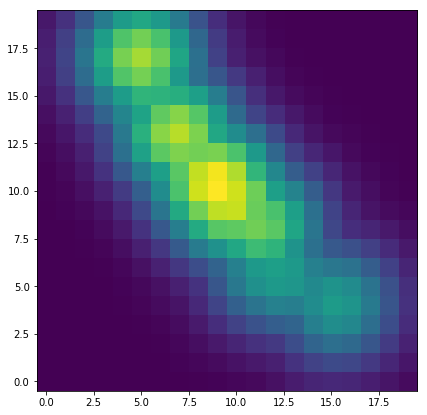
\includegraphics[width=0.6\linewidth]{gridify.png}
\caption{$25 \times 25$ discrete approxmation 离散近似}
\label{fig:gridify}
\end{figure}

So firstly we draw a square in the grid according to the approximated probability, 
and then draw two uniform variable $dX \sim U(0,5-(-1)/100),dY \sim U(0,(6-0)/100)$ 
to determine the position drew by this process.

Repeating the process 10 times, 
we can get size 10 independent sample from the distribution as such Figure~\ref{fig:stateSampleBattle}.

给出离散近似后,首先按离散概率从此二维网格中选一个格子,然后加上均匀分布噪声 
$dX \sim U(0,5-(-1)/100),dY \sim U(0,(6-0)/100)$ ,算出随机到的位置。

重复此过程10次,就可以从这个分布中采样到10个独立的样本,一个特定样本见图~\ref{fig:stateSampleBattle}。


\begin{figure}[ht]
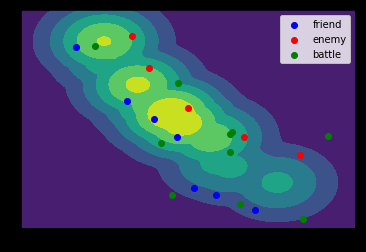
\includegraphics[width=0.6\linewidth]{state_sample_battle.png}
\caption{Ally,enemy,prob, and a sample of battle 敌友军,战役概率与一个特定战役样本}
\label{fig:stateSampleBattle}
\end{figure}

If the positions of enemy is hidden, 
then we can get a instance of problem data as Figure~\ref{fig:stateNoEnemy}.

这时如果把敌人的位置隐去,就可以得到实际推断中所用的数据,如图~\ref{fig:stateNoEnemy}。
如频率主义稻草人式讨论,可以通过比较生成过程隐去的真实值与推断的值来判定推断的效能。

\begin{figure}[ht]
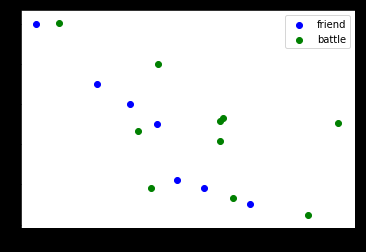
\includegraphics[width=0.6\linewidth]{state_no_enemy.png}
\caption{hide enemy 隐藏敌人后,实际推断时所能看到的信息}
\label{fig:stateNoEnemy}
\end{figure}

\subsection{另一种模型设定}

Although the distribution may satisfy our goal, 
but the $\min$ function will make that gradient-based optmization method difficult to effect 
in those units whose is not nearest to observed battle. 
So a another specification is proposed below to get it done:

First, a differentiable classifier is used to determine the "conflict level" in every point.
Supposing a point is more likely be controled by S side 
if a unit of S side have shortest distance to it, then we can define that the more two control probability 
being close to eachother, the more conflict chance in this point. So the conflict factor is defined by:

尽管这个分布看上去好像还不错,但是$\min$函数使得之后将介绍的三种基于梯度下降的方法无法发挥作用。
如考虑一个敌军备选点如果并没有任何战役点的最近敌军点是它,则它并不能接收到任何梯度信息,
从而无法被优化。所以这里再建立另一种模型:

首先选择一个可微分分类器,它输入友军和敌军位置,判别一个点属于友军和敌军的概率。显然那些难以判别的点
可以被看做冲突可能最大的点,从而可以如此定义坐标$(x,y)$的冲突水平因子:

$$
P_{\text{conflict}}(x,y) = P_\text{ally}(x,y) P_\text{enemy}(x,y) = P_\text{ally}(x,y)(1-P_\text{ally}(x,y))
$$

Where $P_\text{ally}(x,y)$ indicate the probability(belief) of $(x,y)$ being classified 
into ally set given by classifer.

In this paper, we use naive bayes classifer as classifer since it helps gradient computation. 
The classification probability are given by:

这里$P_\text{ally}(x,y)$表示点$(x,y)$被分类器分类为友军的概率。

本文剩余内容使用朴素贝叶斯分配器作为分类器($x,y$坐标为独立的特征)。
它相对容易计算,其意义也易于解释。分类器分类概率被定义为:

$$
P_\text{ally}(x,y) = \frac{
N(x\mid \mu^A_X ,\sigma^A_X) N(y \mid \mu^A_Y, \sigma^A_Y)
}{
N(x \mid \mu^A_X , \sigma^A_X) N(y \mid \mu^A_Y , \sigma^A_Y) + 
N(x \mid \mu^E_X , \sigma^E_X N(y \mid \mu^E_Y , \sigma^E_Y)
}
$$

Where $N(x \mid \mu,\sigma)$ is normal probability density function:

这里$N(x \mid \mu,\sigma)$是正态分布概率密度分布函数:
$$
N(x \mid \mu,\sigma) = \frac{1}{\sqrt{2\pi \sigma^2}} \exp\left(\frac{(x-\mu)^2}{2\sigma^2}\right)
$$

The classifier parameters $\mu,\sigma$ are estimated by normal moment estimation. 

分类器所用的参数$\mu,\sigma$以标准的矩估计法估计得到:

\begin{align*}
\mu_Z^S    &= 1/N^S \sum_{i=1}^N Z_i^S \\
\sigma_Z^S &= 1/N^S (Z_i^S - \mu_Z^S)^2
\end{align*}

Where $Z \in \{ X,Y \}$ and $S \in \{ A,E \}$. $N_S$ is number of units of side $S$.

A living example of classify probability can be seen in Figure~\ref{fig:naivebayes}.

这里 $Z \in \{ X,Y \}$ ,$S \in \{ A,E \}$。而 $N_S$为$S$方的单位数量。

图~\ref{fig:naivebayes} 可视化了各点的分类概率情况。

\begin{figure}[ht]
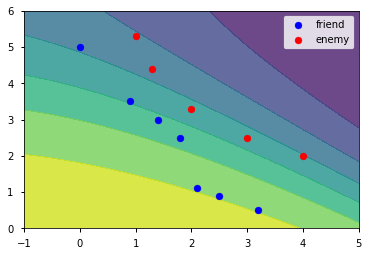
\includegraphics[width=0.6\linewidth]{naivebayes.png}
\caption{naive bayes predict probability coutour map 朴素贝叶斯分配器预测概率等高线图}
\label{fig:naivebayes}
\end{figure}

Then, we define that the less the distance between point and any units(ally or enemy) be,
the more likely the point will occur a battle.

接下来,定义距离因子吸收回之前模型的距离信息。点与最近的单位的距离越小,则越有可能产生一场战斗,
定义为:

$$
P_{\text{distance}}(x,y) = \exp(-\alpha \min_{u} distance)
$$

Where $u$ means any unit. $\min_u distance$ the shortest distance in all possible distance 
between coordinate of unit and $(x,y)$.

So the probability is:

这里$u$意味任意单位。$\min_u distance$所有单位所在点到点$(x,y)$之间的距离中最短者。

故而产生战斗概率为:

$$
P(x,y) = P_{\text{conflict}}(x,y) P_{\text{distance}}(x,y) = 
P_\text{ally}(x,y) P_\text{enemy}(x,y) \exp(-\alpha \min_{u} distance)
$$

Set $\alpha=0.1$, the 2d function can be seen in Figure~\ref{fig:combOne}:

设$\alpha=0.1$,这个二维函数值可见图~\ref{fig:combOne}:

\begin{figure}[ht]
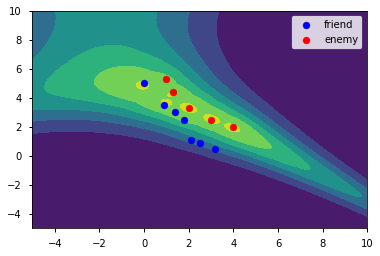
\includegraphics[width=0.6\linewidth]{comb1.png}
\caption{Combining a naive bayes classifier and a smooth distance factor
组合朴素贝叶斯分类器与平滑的距离因子后的战斗概率}
\label{fig:combOne}
\end{figure}

The smooth probability seems good, but the sampled result seems too diffused 
(see Figure~\ref{fig:combTwo}) and if scale is enlarged, 
the problem even worsen (see Figure~\ref{fig:combThree}).
Some parameters tuning are tried but not satisfy the demand. 
So the smooth function family are removed and uniform distribution is employed. 

光滑化概率虽然看起来不错,但是经过实验发现抽出来的样本有点过于分散了(见图~\ref{fig:combTwo})
而如果将考虑区域加大,则情况会变得更糟(见图~\ref{fig:combThree})。
虽然尝试调整参数设定,但没能达成两全其美。故而这个光滑设法又被放弃,
转而将冲突水平和距离直接与对应阈值比较,若没超过就直接设其概率为0的截断设定。

\begin{figure}[ht]
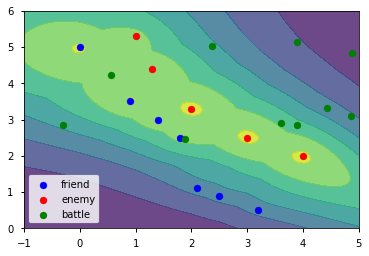
\includegraphics[width=0.6\linewidth]{comb2.png}
\caption{Too diffused sample 过于分散的样本}
\label{fig:combTwo}
\end{figure}

\begin{figure}[ht]
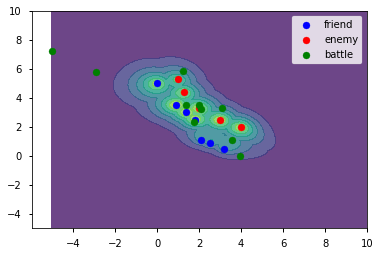
\includegraphics[width=0.6\linewidth]{comb4.png}
\caption{When extend the scale, unrational sample will present inevitably.
当扩大讨论范围后,不合理的样本不可避免地出现}
\label{fig:combThree}
\end{figure}

\subsection{Empolyed setting}

We assign a point constant probability 
if it is greater than conflict threshold and less than distance threshold:

%这段和上面合一起了

$$
P(x,y) \propto
\begin{cases}
1 & P_\text{ally}(x,y) (1-P_\text{ally}(x,y)) > \text{ conflict threshold and }
    \min_{u} distance < \text{conflict threshold} \\
0 & \text{otherwise}
\end{cases}
$$

Figure~\ref{fig:combFive} shows how the unrational sample point is suppressed by the way.

图~\ref{fig:combFive}展示了样本点被强制落在阈值确定的区域内,解决了过于分散的困境。

\begin{figure}[ht]
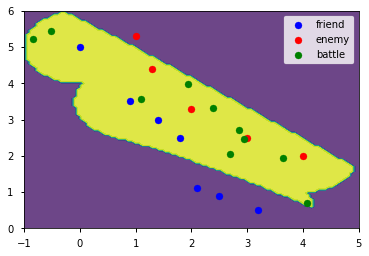
\includegraphics[width=0.6\linewidth]{comb5.png}
\caption{Forced 0 zero probability can suppress the unrational point
强制0概率可以解决不合理点的麻烦}
\label{fig:combFive}
\end{figure}

To get gradient information to proceed optimization, 
rewrite the conditional jump function to "soft" version, 
just like relation of ReLu and softplus in machine learning. 
For example, sigmmoid function $sigm(x) = \frac{1}{1+\exp(-x)}$:

不过这个设定同样有无法传递梯度信息问题,这里采用机器学习常用的“软化”方法(如机器学习把ReLu换成softplus)
来截断函数转为S型函数,这里采用sigmoid函数 $sigm(x) = \frac{1}{1+\exp(-x)}$:

$$
P(x,y) \propto sigm(t (P_\text{ally}(x,y) (1-P_\text{ally}(x,y)) - \theta_0)) sigm(t(-\min_{u} distance + \theta_1))
$$

Where $t$ is "tense" parameter controling the shape of sigmoid, $\theta_0,\theta_1$ are threshold for
conflict level and distance. For $\theta_0=0.2,\theta_1=1.5,t = 10.0$, the result can be show in Figure~\ref{fig:combSix}.

这里 $t$ 是“紧绷度”参数,其控制了sigmoid函数的陡度, $\theta_0,\theta_1$是冲突程度和距离的阈值。
 设 $\theta_0=0.2,\theta_1=1.5,t = 10.0$,其效果可见图~\ref{fig:combSix}.


\begin{figure}[ht]
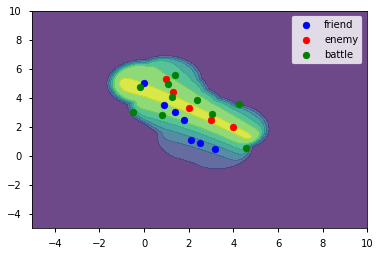
\includegraphics[width=0.6\linewidth]{comb6.png}
\caption{Selected model 基线模型}
\label{fig:combSix}
\end{figure}

The model seems perfect to our demand, following article will use it as baseline model.

后文将使用这个模型和参数设定作为基线模型。

\section{推断的算法和框架}

A bayes inference framework is a programming language or a library that is made to organize the 
programming for model and inference related optmization code.

贝叶斯推断框架是组织模型设定和推断方法的库或者领域特定语言。

\subsection{既有的推断框架}

There're a lot of inference framework such as Stan \cite{carpenter2017stan}, 
pymc\cite{patil2010pymc} and edward \cite{tran2016edward}. 
The core of them are a automated gradient computation library, 
they're stan-math, theano, tensorflow respectively. 

Nevertheless, those except stan are too weak in their ability describing complex probabiliy function.
And the compile time of stan is too long. 
So a light-weight bayes inference library is proposed to fulfill our goal. 
The framework is based on pytorch providing a flexible automated gradient computation lib and 
easy-to-use dynamic computation graph like Chainer.

现在已经很多流行的推断框架,如 Stan \cite{carpenter2017stan},
pymc\cite{patil2010pymc} , edward \cite{tran2016edward}. 
它们的核心是其所基于的自动求导库,这三个对别对应于 stan-math,theano,tensorflow。


\subsection{推断方法和算法介绍}

In this section, three inference method used below sections will be introduced.

这节将介绍三种后文反复使用的推断方法。本文为了推断的灵活起见自己开发了一个被称作bayes-torch的基于
pytorch作为自动求导库的库
\footnote{代码已托管在GitHub并发布在PyPi,参见\url{https://github.com/yiyuezhuo/bayes-torch}},
实现了这三个方法。

\subsubsection{最大后验估计}

Maximum A Posteriori(MAP) is a estimator that maximize the likelihood function 
coporating prior information. Since the task of gradient computation is done by pytorch, 
we can only call the SGD or any other artful NN(neural net)-oriented optimizer to do standard gradient 
descent (take $loss = -likelihood \times prior$) process. See Algorithm~\ref{alg:sgd}.

最大后验估计(MAP)找到使得似然函数和先验概率最大化的点作为估计值。由于梯度计算可以用pytorch自动完成,
这里只需调用SGD或者pytorch提供的其他面向神经网络的优化器(毕竟pytorch本身是用来实现动态神经网络的)
来进行标准的梯度下降(取 $loss = -likelihood \times prior$)过程。见算法~\ref{alg:sgd}。

\begin{algorithm}
\caption{随机梯度下降}
\begin{algorithmic}[1]
\Procedure{SGD}{$\theta,lr,step$} \Comment{$\theta$ 是初始值, $lr$ 更新速率,$step$ 是迭代步数}
    \For{i in 1:step}
        \State $\nabla \gets (\nabla_\theta \log(x,\theta)|_{\theta})$
        \State $\theta \gets \theta - lr \nabla -\theta$
    \EndFor
    \State \textbf{return} $\theta$
\EndProcedure
\end{algorithmic}
\label{alg:sgd}
\end{algorithm}

\subsubsection{变分推断}

Variational inference use simple joint distribution setting to approximate complex 
exact posterior distribution, using Kullback-Leibler(KL) diversity as optimizing target \cite{blei2017variational}. That is:

变分推断使用简单的分布区近似复杂的精确后验分布。它的优化目标是使得变分(近似)分布与原分布的Kullback-Leibler(KL)散度最小化
\cite{blei2017variational},也就是说:

$$
KL(q||p) = E_q \left( \log \frac{q(\theta \mid \mu,\omega)}{p(\theta \mid x)} \right)
$$

Where $p(\theta \mid x)$ is exact posterior distribution. 
$q(\theta)$ is corresponding variational distribution approximating the exact one.
The family of $q(\theta)$ are usually employed as normal distribution, especially $N(\mu,\mathbf{\sigma})$ form.
If $\mathbf{\sigma}=\mathrm{diag}(exp(\mathbf{\omega}))$, 
that is so called meanfield setting we will see it in following content.
%$q(\theta \mid \mu,\omega)$ is corresponding variational distribution approximating the exact one
%and the $\mu,\omega=\log(\sigma)$ means the distribution is in normal family with independent variable(meanfield).
%The $\mu,\omega$ will be omited in following content.

Since it employ variational(approximated) distribution $q(\theta)$ as expectation weight 
instead of exact posterior distribution,
the computation difficulty is relative reduced. But it seems too hard to deal too. 
So we turn to considering evidence lower bound(ELBO) which is lower bound for $\log p(x)$:

这里$p(\theta \mid x)$是精确后验分布。$q(\theta)$是对应的近似精确分布的近似分布。
$q(\theta)$的分布族经常为了计算方便而选为正态分布,即$N(\mu,\mathbf{\sigma})$形式。
如果协方差矩阵可以视作对角矩阵,即$\mathbf{\sigma}=\mathrm{diag}(exp(\mathbf{\omega}))$,
这就是所谓采用了平均场设定的变分推断,它在也许不合理的移去随机参数之间的关系的同时也极大减少了参数个数并
加速了算法。

由于采用了近似分布而非精确后验分布作为权重计算期望,解析上的计算难度稍有下降。
不过依然不好计算,故而转而优化证据下界(ELBO),它的下界之名得自它是$\log p(x)$的下界:

\begin{align*}
\log p(x) &= \log \int_\theta p(x,\theta) = \log \int_\theta p(x,\theta) \frac{q(\theta)}{q(\theta)} = \log \left( E_q \frac{p(x,\theta)}{q(\theta)} \right)  \\
          &\ge E_q (\log p(x,\theta)) - E_q(\log q(\theta)) = \mathrm{ELBO}
\end{align*}

The relation of KL diversity and ELBO can be show:

KL散度和ELBO的关系如下:

\begin{align*}
KL(q(\theta) || p(\theta \mid x)) &= E_q \log \frac{q(\theta)}{p(\theta \mid x)}  \\
                                  &= E_q \log q(\theta) - E_q \log p(\theta \mid x) \\
                                  &= E_q \log q(\theta) - E_q \log p(\theta,x) + E_q \log p(x) \\
                                  &= -(E_q \log p(\theta,x) -E_q \log q(\theta)) + \log p(x) \\
                                  &= -\mathrm{ELBO} + \log p(x)
\end{align*}

So we can maximizing ELBO to minimizing KL diversity. 
To do the optimization, the tradition variational inference method, 
Coordinate ascent variational inference (CAVI) algorithm,
require a analytic conditional expectation $E_{-j}(\log p(\theta_j \mid \mathbf{\theta}_{-j},\mathbf{x}))$. 
It's annoy when lazy statistician aware that he can do sampling to
reach same goal without any of such brain exhausted brain challenges. 

The Automatic differentiation variational inference (ADVI) is presented by 
\cite{kucukelbir2017automatic} and \cite{kucukelbir2014fully} to fix it. 
The core of the algorithm is to use random integral to approximate a hard-to-deal expectation.

Algorithm~\ref{alg:advi} is a simplified version from \cite{kucukelbir2017automatic}, benefited that we don't need transform
the support of restricted variable to unconstrained space.

所以可以最大化ELBO来最小化KL散度。做这个优化的传统变分推断算法,所谓的坐标提升变分推断(CAVI)算法
要求解析的计算条件期望$E_{-j}(\log p(\theta_j \mid \mathbf{\theta}_{-j},\mathbf{x}))$。
这并不是个如同自动求导一样容易自动解决的问题,这使得变分推断没有采样法这种开箱即用的方法一样流行。

为了回避解析计算,\cite{kucukelbir2017automatic}与\cite{kucukelbir2014fully}提出自动微分变分推断(ADVI)。
这个算法的核心是蒙特卡洛法计算一个复杂期望,如算法~\ref{alg:advi}所示。该算法是
\cite{kucukelbir2017automatic}的算法的简化版本,
原文讨论的更一般的非自由取值变量的变换的相应处理等由于本文不需要并没有被实现。

\begin{algorithm}
\caption{自动微分变分推断(平均场+无变换)}
\begin{algorithmic}[1]
\Procedure{ADVI}{$\mathbf{\mu},\mathbf{\omega},lr,M,step$}  \Comment{$\mathbf{\omega}$ 是初始值, M 蒙特卡洛积分的采样个数}
    \For{$s$ in $1:step$}
        \State $\hat{\nabla} \gets \mathbf{0}$
        \State $\mathbf{\eta} \sim N(\mathbf{0},\mathbf{I}) $ \Comment{从多元标准正态分布中采样}
        \For{$i$ in $1:M$} 
            \State $\hat{\theta} \gets (\mathbf{\eta}_i \exp(\mathbf{\omega}_i)) + \mathbf{\mu}_i$
            \State $\hat{\nabla} \gets \hat{\nabla} + (\nabla_\theta \log p(x,\theta)|_{\hat{\theta}})$
        \EndFor
        \State $\hat{\nabla} \gets \hat{\nabla} / M$
        \State $\mu \gets \mu + lr \hat{\nabla}$
        \State $\omega \gets \omega + lr \hat{\nabla} \mathbf{\eta}^T \mathrm{diag}({\exp(\omega)}) + \mathbf{1}$
    \EndFor 
    %\textbf{return} $\mathbf{\mu},\mathbf{\omega}$
    \State \Return $\mathbf{\mu},\mathbf{\omega}$
    %\State 
\EndProcedure
\end{algorithmic}
\label{alg:advi}
\end{algorithm}

The ADVI use noised gradient to find posterior expect that is equal to MAP(with more low effiecency),
 and collect gradient shock and concussion to estimate posterior variance.
 
In this paper, meanfield normal approximation is employed. That is:

ADVI使用带噪声的梯度找到后验期望这一部分有点像降低效率版的MAP,不过这个噪声降低了期望的“估计效率”
的同时也提供了估计方差的机会。

本文使用平均场设定后,后验概率看起来像:

$$
p(x^E_1,\dots,x^E_{N_E},y^E_1,\dots,y^E_{N_E} \mid D) \sim 
N((\mu_{X^E_1},\dots,\mu_{y^E_{N_E})^T},\mathrm{diag}(\sigma_{X^E_1},\dots,\sigma_{y^E_{N_E}}))
$$

Where $p(x^E_i \mid D) \sim N(\mu_{x^E_i},\sigma_{x^E_i}^2)$. 
Such $\mu_{x^E_i},\sigma_{x^E_i}^2)$ are called variational(approximated) parameters. 
it's called meanfield since the covariace matrix is a diagonal matrix, 
excluding all of correlation between randomized parameters.

条件独立性蕴含$p(x^E_i \mid D) \sim N(\mu_{x^E_i},\sigma_{x^E_i}^2)$,
其中$D$指模型中的已知数据,即给定的友方军队位置和战役位置。而诸如$\mu_{x^E_i},\sigma_{x^E_i}^2)$
被称为变分(参数精确后验分度的近似分布的)参数。

\subsubsection{采样法}

Variational inference is only a approximating method, 
sampling from posterior distribution directly is exact but resource expensive method. 
Classic Hasting-Metropolis method rely on a proposed distribution manually specified by statistician
and suffer bad converge effciency. 
The Hamiltonian Monte Carlo \cite{hoffman2014no} (See Algorithm~\ref{alg:hmc}) can be employed to improve the effciency,
using gradient information instead of proposed distribution to give next step in random walking. 

变分推断只是近似方法,从后验分布中直接采样开销很大但是是精确方法(虽然它的保证收敛并没有看上那么有用)。
经典的Hasting-Metropolis法要使用手动指定的proposed分布,而且收敛效率不佳。哈密顿蒙特卡洛
(HMC,\cite{hoffman2014no},见算法~\ref{alg:hmc})效率更高,且不需要受手动指定proposed分布之苦,
符合各框架热衷于培育的开箱即用统计风格。

\begin{algorithm}
\caption{哈密顿蒙特卡洛}
\begin{algorithmic}[1]
\Procedure{HMC}{$\theta_0,\epsilon,L,step$} \Comment{$L$ ,$\epsilon$ 是 leap-frog过程的参数}
    \For{$i$ in $1:step$}
        \State $r_0 \sim N(0,I)$
        \State $\theta_i \gets \tilde{\theta} \gets \theta_{i-1}$
        \State $\tilde{r} \gets r_0$
        \For{$l$ in $1:L$} \Comment{leap-frog过程}
            \State $\tilde{r} \gets \tilde{r} + (\epsilon/2) \nabla_\theta P(X,\theta)|_{\tilde{\theta}}$
            \State $\tilde{\theta} \gets \tilde{\theta} + \epsilon \tilde{r}$
            \State $\tilde{r} \gets \tilde{r} + (\epsilon/2) \nabla_\theta P(X,\theta)|_{\tilde{\theta}}$
        \EndFor
        \State $\alpha \gets \min \left\{ 1, \frac{\exp(P(x,\tilde{\theta})-\frac{1}{2}\tilde{r}\cdot\tilde{r})}{\exp(P(x,\theta_{i-1})-\frac{1}{2}r_0\cdot r_0)} \right\}$
        \State $u \sim Uniform(0,1)$
        \If{$u \le \alpha$}
            \State $\theta^i \gets \tilde{\theta}$
        \EndIf
    \EndFor
    \State \Return $\theta$
\EndProcedure
\end{algorithmic}
\label{alg:hmc}
\end{algorithm}

HMC follow the same way as ADVI using gradient pulse and bounce.

HMC and other sampling method return a "trace" sample that can be used 
to build empirical posterior distribution. In this paper, the trace almost always been see as
parameters of normal distribution to compare to VB(ADVI) thougn it drop the main advantage of sampling method.

HMC使用与ADVI类似的利用梯度冲击和震荡收集方差信息。

HMC和其他采样法会返回随机游走轨道,这个轨道可以近似的看做精确后验分布的采样样本,所以可以用来计算
其他参数或者生成经验分布函数之类的。后文并不会利用采样法的精确特征,基本只用上它的期望和方差,类似于ADVI。

\section{Inference experiments 推断实验}

\subsection{Enemy position detecting 敌军位置探测}

The situation (see Figure~\ref{fig:expState}) will be used as inference experiment data.

如图~\ref{fig:expState}所示的局势会被用在下面的推断实验中。

\begin{figure}[ht]
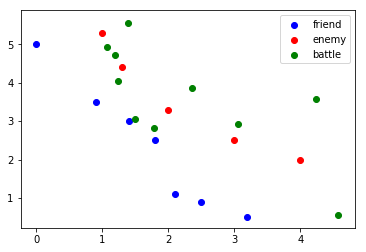
\includegraphics[width=0.6\linewidth]{exp_state.png}
\caption{Given situation}
\label{fig:expState}
\end{figure}


\subsubsection{MAP}

Firstly, if flat prior is used (only provide likelihood), the MAP result is Figure~\ref{fig:MAPone}.

首先,如果使用均匀先验(等价于只有似然函数起作用),MAP的估计结果可见于图~\ref{fig:MAPone}。

\begin{figure}[ht]
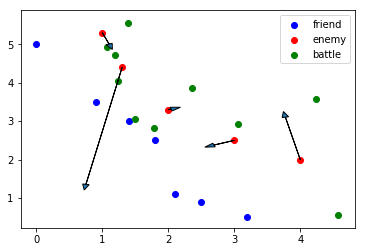
\includegraphics[width=0.6\linewidth]{MAP1.png}
\caption{均匀先验下的MAP}
\label{fig:MAPone}
\end{figure}

The arrowtail indicate the "true" position of enemy(though it can't be seen), 
the arrowhead indicate the estimated position of enemy for MAP. As we can see,
a enemy is pulled to the back of ally units to maximize probability, it seems overfit anyway.
We can utilize the advatage of bayes framework, adding a prior \footnote{Or regulation term, but I
prefer the probability meaning offered by bayes.}:

箭头尾指向对应敌军的“真实位置”(对推断来说不可见),箭头头指向MAP估计的敌军位置。正如所见,
有一个敌军单位的估计位置被拉到友军后方以最大化概率,很明显的过拟合的标志。
贝叶斯框架解决这种问题的标准方式就是引入先验
\footnote{或者叫机器学习的规范项之类的,但是看起来贝叶斯的概率解释更优雅一些。},如:

$$
P_{\text{enemy}}(x,y) = \exp(sigm(t((x+y) - \alpha)))
$$

Where $t$ is tense parameter for enemy position,
$\alpha$ is corresponding threshold. We set $t=5.0,\alpha=5.0$
for illustration below.

The new joint probability with the diagonal prior is:

这里$t$是敌军位置的紧绷度参数。$\alpha$是对应的阈值。这里设$t=5.0,\alpha=5.0$。

由于该先验给对角线右上的区域以偏好,所以称作对角先验。加上对角先验后的联合概率函数看起来像:

\begin{align*}
\log p(\mathbf{x}^E,\mathbf{y}^E) &= \sum_{i=1}^{N_B} \log sigm(t (P_\text{ally}(x^B_i,y^B_i)(1-P_\text{ally}(x^B_i,y^B_i)) - \theta_0)) \\
                                  &+ \sum_{i=1}^{N_B} \log sigm(t(-\min_{u} distance(x^B_i,y^B_i) + \theta_1)) \\
                                  &+ \sum_{j=1}^{N_E} sigm(t((x^E_j+y^E_j) - \alpha))
\end{align*}

Where $N_B,N_E$ are number of battle and enemy,$x^B_i,y^B_i$ is coordinate of battle $i$, $x^E_j,y^E_j$
is coordinate of enemy $j$.

The result of MAP on the new probability function looks better as shown in the Figure~\ref{fig:MAPtwo}.

这里$N_B,N_E$是战役和敌人单位的个数。$x^B_i,y^B_i$是第$i$个战役的坐标。$x^E_j,y^E_j$是第$j$个敌人的坐标。

从图~\ref{fig:MAPtwo}中可以看出,加上对角先验后的MAP结果不再出现那种过拟合情况。

\begin{figure}[ht]
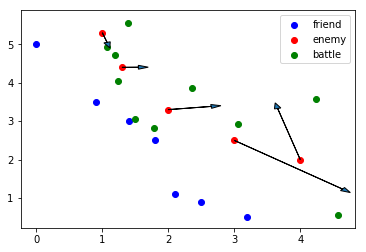
\includegraphics[width=0.6\linewidth]{MAP2.png}
\caption{对角先验下的MAP}
\label{fig:MAPtwo}
\end{figure}

\subsubsection{Sampling and Variational inference 采样和变分推断}

Point estimation is not enough since it can't give uncertain information about the estimation.
Tough exact posterior may fix it but it's hard to compute and represent. Two ways in bayes inference 
to do it are sampling and variational inference(VI). The former one generate a "trace" which can be thought
as a sample taken from exact posterior, the trace may contitude empirical distribution or reveal 
attribution of the random parameter. The VI is faster but lack exact attribution.

The two results of VI in flat prior and new diagonal prior can be seen in Figure~\ref{fig:VI}.
The two results of sampling can be seen in Figure~\ref{fig:samping}.

点估计本身没有给出关于估计的不确定性信息。尽管精确后验分布的参数可以直接给出但是难以计算。
贝叶斯推断中两种解决方式就是采样和变分推断(VI)。前者产生一个与精确后验相关的随机游走轨迹,其可以看做
从后验中采样出来的,精确但是效率低下,而变分推断快得多但是理论上仅是近似。

\begin{figure}[ht]
  \begin{subfigure}[b]{0.45\linewidth}
    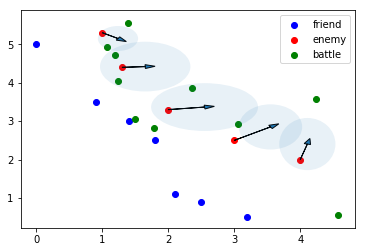
\includegraphics[width=\linewidth]{VI11.png}
    \caption{变分推断+均匀先验例一}
  \end{subfigure}
  \begin{subfigure}[b]{0.45\linewidth}
    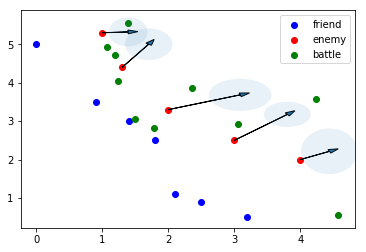
\includegraphics[width=\linewidth]{VI12.png}
    \caption{变分推断+对角先验例一}
  \end{subfigure}
  \begin{subfigure}[b]{0.45\linewidth}
    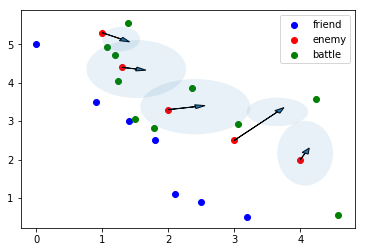
\includegraphics[width=\linewidth]{VI21.png}
    \caption{变分推断+均匀先验例二}
  \end{subfigure}
  \begin{subfigure}[b]{0.45\linewidth}
    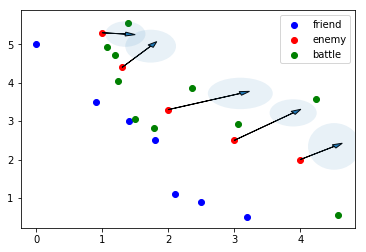
\includegraphics[width=\linewidth]{VI22.png}
    \caption{变分推断+对角先验例二}
  \end{subfigure}
  \caption{变分推断拟合结果}
  \label{fig:VI}
\end{figure}

\begin{figure}[ht]
  \begin{subfigure}[b]{0.45\linewidth}
    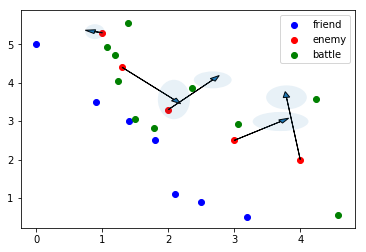
\includegraphics[width=\linewidth]{Sampling11.png}
    \caption{哈密顿蒙特卡洛+均匀先验例一}
  \end{subfigure}
  \begin{subfigure}[b]{0.45\linewidth}
    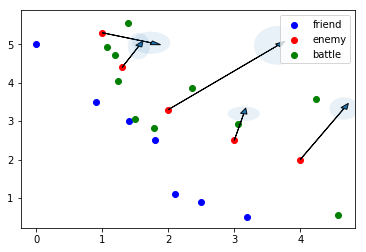
\includegraphics[width=\linewidth]{Sampling12.png}
    \caption{哈密顿蒙特卡洛+对角先验例一}
  \end{subfigure}
  \begin{subfigure}[b]{0.45\linewidth}
    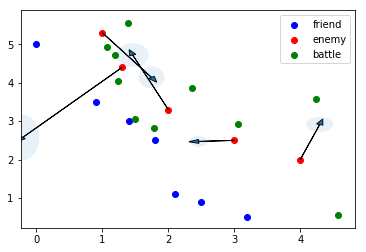
\includegraphics[width=\linewidth]{Sampling21.png}
    \caption{哈密顿蒙特卡洛+均匀先验例二}
  \end{subfigure}
  \begin{subfigure}[b]{0.45\linewidth}
    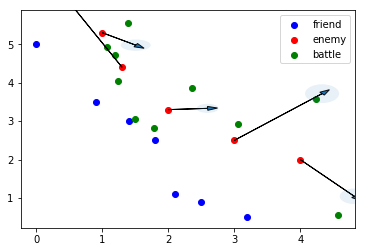
\includegraphics[width=\linewidth]{Sampling22.png}
    \caption{哈密顿蒙特卡洛+对角先验例二}
  \end{subfigure}
  \caption{采样法拟合结果(100次采样)}
  \label{fig:samping}
\end{figure}

Where the coordinate of ellipses indicate the expectation of those posterior distribution,
and the radius of ellipses indicate the standard deviation(sd) of axis x and y in every latent enemy point.
So those ellipse can be seen as a rough approximation for posterior distribution 
hidden in trace or variational distribution, though those two are not exact posterior too.

The HMC result seems inconsisitency, implying the converge fail. Though increasing sample size may be
solution(see Figure~\ref{fig:SamplingTen}). But just like we are not content to a NP-hard solver and claim that it only need more time,
sampling seems too weak in this problem.

图中的椭圆的中心表示拟合的后验分布(以参数化正态分布或轨迹的经验分布表示)$x,y$的期望,
椭圆的两轴长表示拟合的后验分布的$x,y$的标准差。故而这些椭圆可以看成对计算得近似后验分布的一个粗略表示。

图中可以看到哈密顿蒙特卡洛的拟合结果看起来不能保持一致,这意味着随机游走未充分收敛。
扩大样本量可以稍微解决这个问题(10倍样本结果见图~\ref{fig:SamplingTen})。但是即使是100个样本,
在这个问题中都已经很慢了,所以后文使用的都是变分推断法,而不用采样法。

\begin{figure}[ht]
  \begin{subfigure}[b]{0.45\linewidth}
    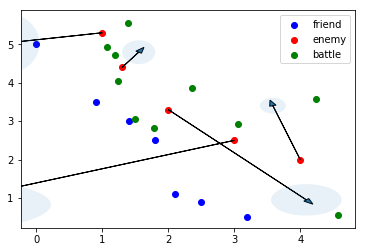
\includegraphics[width=\linewidth]{Sampling31.png}
    \caption{哈密顿蒙特卡洛+均匀先验例一}
  \end{subfigure}
  \begin{subfigure}[b]{0.45\linewidth}
    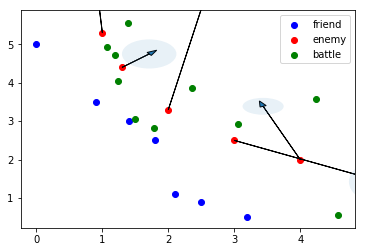
\includegraphics[width=\linewidth]{Sampling32.png}
    \caption{哈密顿蒙特卡洛+对角先验例一}
  \end{subfigure}
  \begin{subfigure}[b]{0.45\linewidth}
    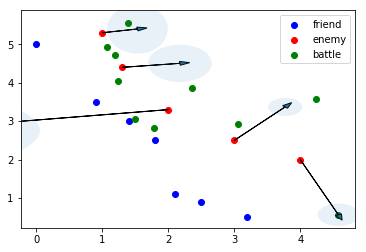
\includegraphics[width=\linewidth]{Sampling41.png}
    \caption{哈密顿蒙特卡洛+均匀先验例二}
  \end{subfigure}
  \begin{subfigure}[b]{0.45\linewidth}
    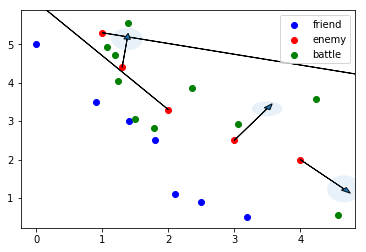
\includegraphics[width=\linewidth]{Sampling42.png}
    \caption{哈密顿蒙特卡洛+对角先验例二}
  \end{subfigure}
  \caption{采样拟合结果(1000次采样)}
  \label{fig:SamplingTen}
\end{figure}

\subsection{Mutiple enemy number setting 变化敌人数量设定}

The above estimation is based on "true" number of enemy. Let we test its stability. 
What happen if the given number of number of enemy is wrong? The Figure~\ref{fig:bigVb} 
show the result, that flat prior seems well while diagonal prior may may be dominated by 
the prior. But it depict what we want in general.

上面的估计都基于“真实”的敌人数量。为了讨论此算法的稳定性,特别是实际不知道敌人确切数量,
乃至给出的数量与实际数量偏差很大时,算法会给出什么结果?图~\ref{fig:bigVb}展示了不同数量设定下的
结果(初始值以真实值插值而来)。可见均匀先验的结果就看起来不错,而对角先验有点过于被先验支配了。
不过总的来说变化敌人数量反而可以证明本算法的有效性。

\begin{figure}[ht]
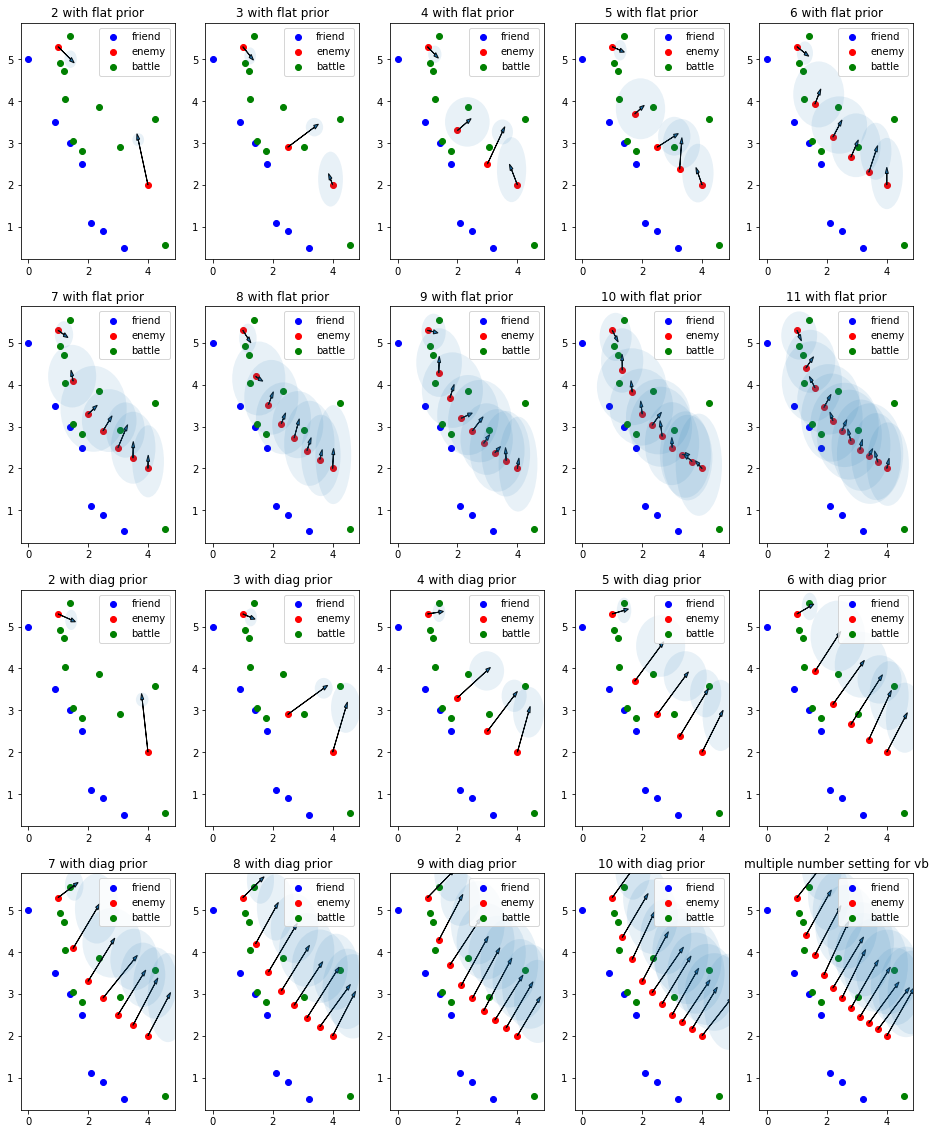
\includegraphics[width=0.99\linewidth]{big_vb.png}
\caption{变动数量时的近似结果}
\label{fig:bigVb}
\end{figure}

\subsubsection{The density of probabity of existence of enemy estimation 敌人存在性概率密度估计}

The one of advantage of VB is that it make computation of probability of specific region very easy.
The probability of exist of enemy in a given region $[x,x+dx]\times[y,y+dy]$ can be given by:

这里采用正态分布族的变分推断的一大好处就是计算特定敌军单位在特定区域的后验概率十分方便。
从而可以直接计算出出区域中存在任意敌军单位的概率:

\begin{align*}
pe(x,y,dx,dy) = 1 - \prod_i (
& (1-(\Phi(x+dx - \mu_{X^E_i})/\sigma_{X^E_i}) -  (\Phi(x - \mu_{X^E_i})/\sigma_{X^E_i})) \\
& (1-(\Phi(y+dy - \mu_{Y^E_i})/\sigma_{Y^E_i}) -  (\Phi(y - \mu_{Y^E_i})/\sigma_{Y^E_i}))
)
\end{align*}

Where $\Phi(x)$ is standard cumulative probability function:

这里$\Phi(x)$是标准正态分布累积分布函数:

$$
\Phi(x) = \int_{-\infty}^x \frac{1}{\sqrt{2\pi}} \exp\left(\frac{x^2}{2}\right)
$$

And $\mu^X_i$ is the expect parameter of normal approximated posterior probability of ith enemy.
The three other are same.

The existence density(approximated) is defined:

而$\mu_{X^E_i}$是第$i$个敌人的近似后验分布的正态期望参数,另外几个类似。

以此可以近似地计算定义出存在密度:

$$
pe(x,y) = pe(x-\epsilon,y-\epsilon,2\epsilon,2\epsilon)/(4 \epsilon^2)
$$

Where $\epsilon$ is a small number, in there $\epsilon=0.01$. 
The two example can be seen in Figure~\ref{fig:existDensity}. 
The comparing result can be seen in seen in Figure~\ref{fig:bigVbExist}.

其中$\epsilon$是一个足够小的数,在这取$\epsilon=0.01$。两个数量设定的计算的结果
可见等高线图~\ref{fig:existDensity}。类似上面比较各个数量的结果见图~\ref{fig:bigVbExist}。

\begin{figure}[ht]
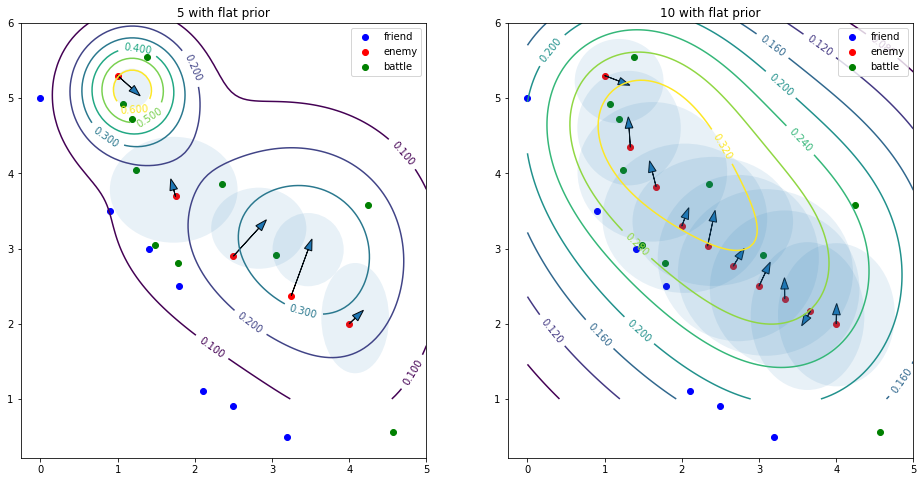
\includegraphics[width=0.99\linewidth]{exist_density.png}
\caption{两个数量设定下的存在概率密度估计}
\label{fig:existDensity}
\end{figure}


\begin{figure}[ht]
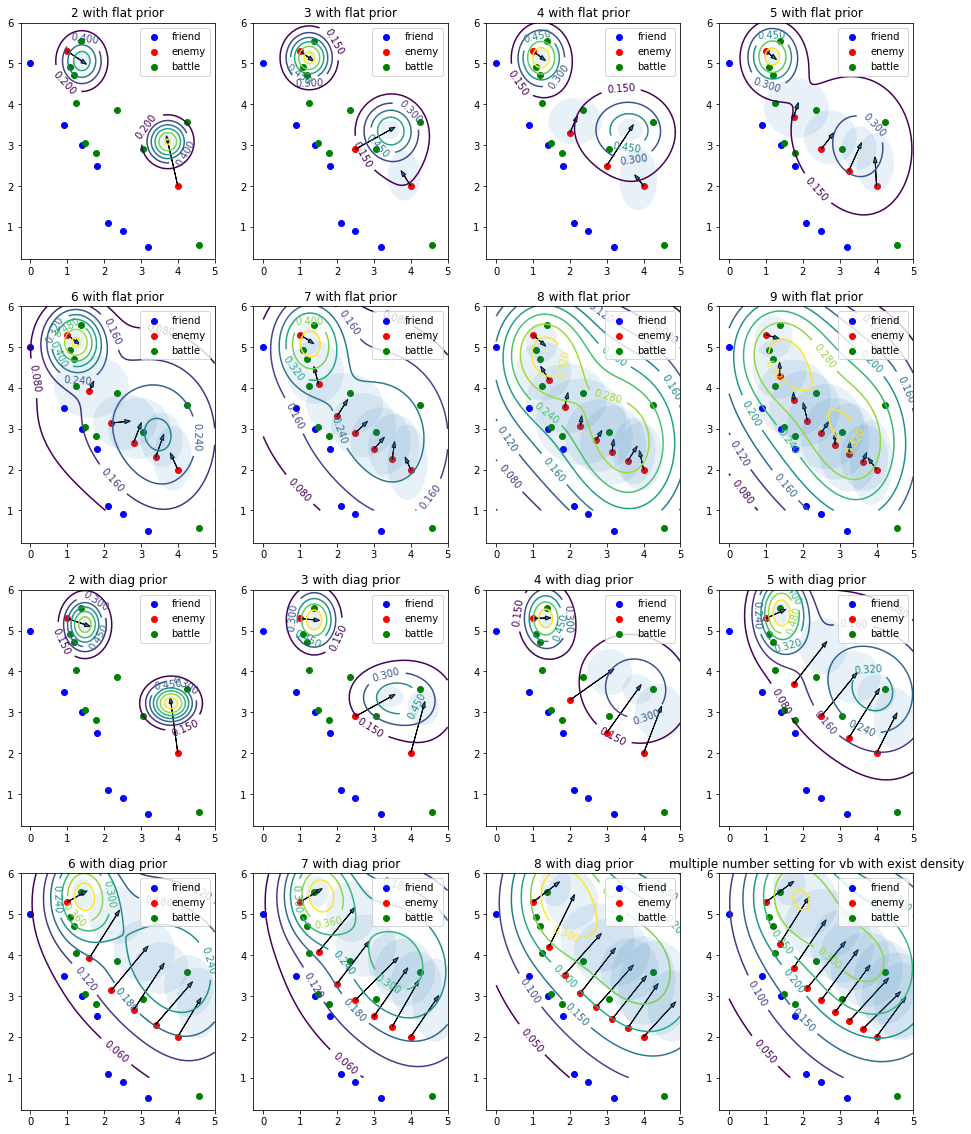
\includegraphics[width=0.99\linewidth]{big_vb_exist_prob.png}
\caption{多个数量设定下的存在概率估计}
\label{fig:bigVbExist}
\end{figure}



\section{Extention: Enemy movement detecting 扩展:敌方运动检测}

Considering ally,enemy,battles have not only positions, but also have timestamp. In another word,
enemy and ally may move in a time range, how do we infer the movement?

Interestingly, the model requires only a bit of modifications to integrate the new specification.

Assurming the time begin at $0$ and end at $1$, and enemy have uniform motion in constant speed.
So the parameters$x^E_i$ can be rewritten as $x^E_i(t) = (1-t)x^E_i(0) + tx^E_i(1)$, 
where $x^E_i(0),x^E_i(1)$ means the positions of ith enemy in time 0 and 1 respectively, and so on.
They are new parameters. The other structual probability function almost keep its original form.

First, assurming $x^E_i(0),y^E_i(0)$ are known and $x^E_i(1),y^E_i(1)$ are unknown.
A instance of inference is shown in Figure~\ref{fig:bkeu}. 
Where arrowtail indicate the known begin point.
The one of two arrowhead surrounded by sd ellipse is estimated $t=1$ coordination expectation. 
The another one is "true" target point.

考虑友军,敌军,战役不仅有位置信息,还有关于何时在何地的时间信息,即敌友军可以在一个时间段内运动
并在一些时间发生战斗\footnote{这里发生时间和次数的随机过程化似乎更有必要了,然而为了简化这里两个都是给定的}
,如何推断运动呢?得益于模型的设定方式,仅需一点改造以上模型就可以用来推断运动。

假定时间开始于$0$并终结于$1$,而敌我双方均以固定的速度(每个单位可以不同)进行匀速运动。故而之前的
参数$x^E_i$可被重写为$x^E_i(t) = (1-t)x^E_i(0) + tx^E_i(1)$。这里$x^E_i(0),x^E_i(1)$是取代原先参数的两个
新参数,表示敌人单位在时间0,1时的位置。其他的几个随机参数或数据也类似如此改变(友军被钦定了额外的运动方式,
在本例中友军都在向“前”运动)。

首先,假定敌军期初位置$x^E_i(0),y^E_i(0)$已知而末期位置$x^E_i(1),y^E_i(1)$未知,
推断的结果可见图~\ref{fig:bkeu}。这里箭头尾表示已知的初始点,
有椭圆包着的那个箭头头坐标表示估计的结果(类似前面,坐标指期望,长短半径场指两轴上的标准差)。
另外一个箭头是“真实”期末点。

\begin{figure}[ht]
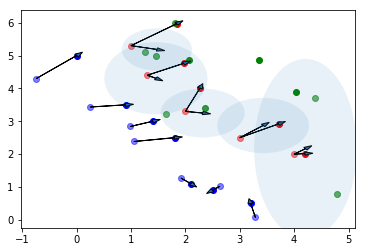
\includegraphics[width=0.4\linewidth]{bkeu.png}
\caption{运动推断:$t=0$已知而$t=1$未知}
\label{fig:bkeu}
\end{figure}

The following Figure~\ref{fig:bueu} show the situation in which $t=0,1$ situation are both unknown
\footnote{Note they're not in same data set.}. Where the arrowtail of first arrow is "true" begin
point, the middile point is estimated posterior expect of the point at $t=0$, the arrowhead of second arrow
is estimated posterior expect of the point at $t=1$.

图~\ref{fig:bueu}显示了当$t=0,1$时敌人的位置都未知时的推断结果\footnote{注意它们没用同一个数据}。
连续的两个箭头的箭头尾出指向真实初始点,中点表示估计的期初点位置坐标的后验期望,
箭头头是估计的期末点位置坐标的后验期望。

\begin{figure}[ht]
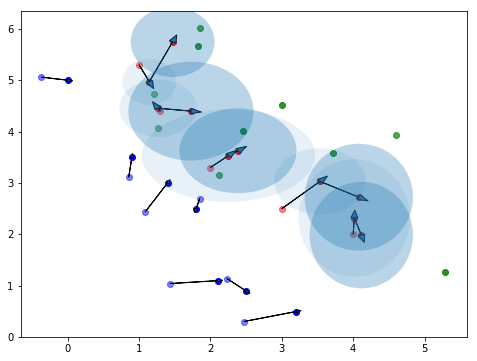
\includegraphics[width=0.6\linewidth]{bueu.png}
\caption{运动推断:$t=0$与$t=1$时敌人位置都未知}
\label{fig:bueu}
\end{figure}

The prior that give punishment to too long moving range also are useful and easy to implement. 
But the dataset that can highlight the advantage don't be constructed yet subject to time limit.
So it will be skiped.

注意这个模型对可能出现的超长运动没有进行先验的惩罚,受制于时间因素,由于算法在这个数据上效果还不错
就没有专门构造个数据去验证这类先验设定的效果了。

\section{Extention: Dealing complex position distribution. 扩展:处理复杂的复杂的分布形状}

The above contents are based on similar distribution, a curve can divide ally and enemy easily.
What will happen if the shape become complex and hard to capture for "one center" bayes naive classifer?

上面讨论的基本都基于那个很容易给出一条曲线将两组点分开的数据,
从而模型中插入的极其简化的朴素贝叶斯分类器都能充分发挥其效能。下面将测试一些其他的形状。

\subsection{Circle 圆形}

The "true" position is droped. This section will contain only "initialization value"
(In above content, "true position" play also initialization value role.). 
The Figure~\ref{fig:circleIteration} show the circle setting with flat prior, 
showing also a nice iteration convege process .

这里将友军位置设为圆形的,战役的位置设定成敌军将友军包围所能产生的,但敌军位置本身不给定,
从而迭代初始值不像之前那样设成真实值而设成随机值。如果这些点可以自动移动到外围的话就可以验证
算法的有效性。而迭代结果如图~\ref{fig:circleIteration}所示,仅仅需要均匀先验而不需要给定
敌军在外部的先验就可以收敛到比较恰当的位置上。

\begin{figure}[ht]
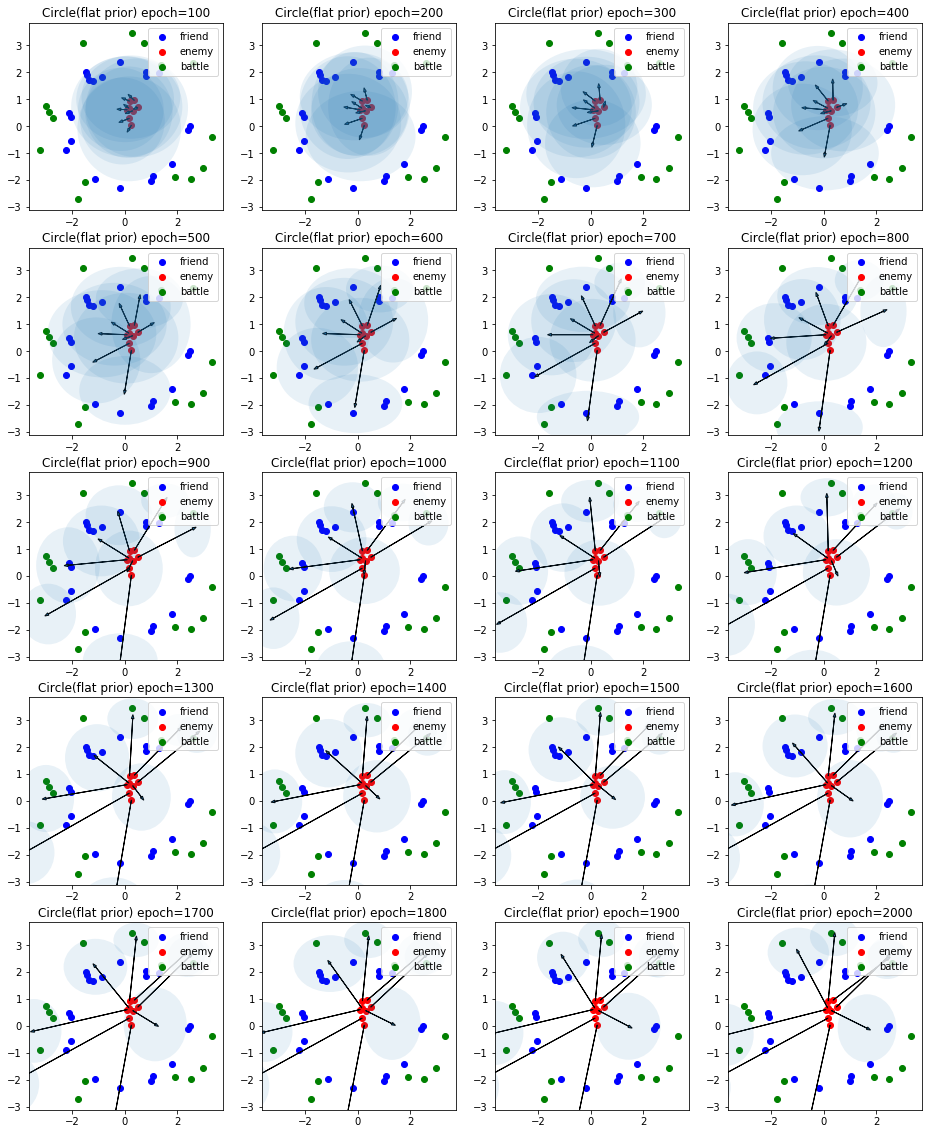
\includegraphics[width=0.99\linewidth]{circle_iteration.png}
\caption{Iteration process for circle setting with flat prior and random initialization
均匀先验+圆形设定+随机初始化下的迭代收敛过程}
\label{fig:circleIteration}
\end{figure}

\subsection{Case study: The battle of Gettysburg 案例研究:葛底斯堡战役}

Now, it's the time to abandon the globular chicken in vacuum loved by physicists.
The Figure~\ref{fig:gettysburg} show the map and corresponding data of the battle of Gettysburg in second day.
The data only capture the division(NATO:XX) and bridge brigade(NATO:X) in the map.
\footnote{You may aware the top right corner is not matched well. 
That is because The data depict state in morning and the map draw the situation in afternoon, the main battle time.
So it miss the march time the former one may infer.}
The confederate army have less number of divisions since the size of the divisions of CSA are more big.
The data is from HPS great wargame "Civil war:Gettysburg". 
The data used are listed in the Table~\ref{tab:Confederate} and \ref{tab:Union}, in which strength 
is number of unit that is not used in the model yet and will be used in later section as weight.

本节不再使用前面使用的真空中的球形鸡来验证模型,而直接使用真实战例的数据。图~\ref{fig:gettysburg}
展示了葛底斯堡战役第二天的战场示意图和单位位置的抽象数据,数据分别标出了旅级单位的分布和师级单位的分布,
下面的推断使用师级单位,不过旅级的看起来更连续一些\footnote{你可能会注意到两图在右上角并不完全一致,
这是因为战场示意图是战斗过程的图,而散点图则是机动到进攻阵地前的确切位置}。数据来自HPS兵棋
“内战系列:葛底斯堡”,此外还有一个人数表,见表~\ref{tab:Confederate}与表~\ref{tab:Union}。
人数将作为后面的将人数考虑进来的模型的权重。另外可从人数上看出联邦军的师规模比南方邦联军小,
所以对所有单位使用相同的参数可能并不十分恰当(在前面时可以假定各单位同质回避这个问题,
然而这里显然不同质)。

\begin{table}
\parbox{.45\linewidth}{
\begin{tabular}{lrrr}
\toprule
{} &  strength &    x &    y \\
\midrule
Heth's Div     &      4628 &  2.4 &  4.8 \\
McLaws' Div    &      6762 &  2.9 &  1.0 \\
Hood's Div     &      6957 &  3.3 &  0.1 \\
Anderson's Div &      6686 &  3.5 &  2.8 \\
Pender's Div   &      5080 &  3.6 &  3.7 \\
Rodes' Div     &      5202 &  5.0 &  4.2 \\
Early's Div    &      4572 &  6.0 &  3.9 \\
Johnson's Div  &      6012 &  7.2 &  4.5 \\
\bottomrule
\end{tabular}
\caption{Confederate oob}
\label{tab:Confederate}
}
\hfill
\parbox{.45\linewidth}{
\begin{tabular}{lrrr}
\toprule
{} &  strength &    x &    y \\
\midrule
2nd D (Humphreys)   &      4913 &  4.2 &  1.7 \\
1st Div (Birney)    &      5008 &  4.5 &  0.8 \\
2nd Div (Gibbon)    &      3558 &  5.1 &  2.3 \\
3rd Div (Hays)      &      3622 &  5.2 &  2.6 \\
1st Div (Caldwell)  &      3303 &  5.2 &  1.8 \\
3rd Div (Schurz)    &      1633 &  5.3 &  3.1 \\
2nd Div (Steinwehr) &      2264 &  5.4 &  2.9 \\
3rd Div (Doubleday) &      2922 &  5.4 &  2.7 \\
1st Div (Barlow)    &      1475 &  5.5 &  3.1 \\
2nd Div (Robinson)  &      1311 &  5.5 &  2.6 \\
1st Div (Wadsworth) &      1697 &  6.2 &  3.0 \\
2nd Div (Geary)     &      3851 &  6.2 &  2.8 \\
1st Div (Williams)  &      4698 &  6.3 &  2.1 \\
2nd Div (Ayres)     &      3990 &  6.6 &  1.6 \\
1st Div (Barnes)    &      3411 &  6.7 &  1.7 \\
3rd Div (Crawford)  &      2842 &  6.8 &  1.6 \\
3rd Div (Newton)    &      4729 &  7.3 &  0.8 \\
1st Div (Wright)    &      4181 &  7.4 &  1.2 \\
2nd Div (Howe)      &      3548 &  9.3 &  0.0 \\
\bottomrule
\end{tabular}
\caption{Union oob}
\label{tab:Union}
}
\end{table}

Following we assurm the position of army of Union and battle are known but CSA not.

下面假定联邦军的位置已知而南方邦联军的位置位置(即南方邦联军等价于前面的敌军)。

\begin{figure}[ht]
  \begin{subfigure}[b]{0.49\linewidth}
    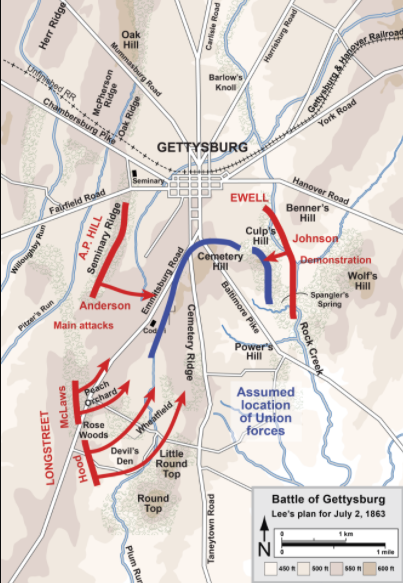
\includegraphics[width=\linewidth]{gettysburg-map.png}
    \caption{葛底斯堡战役第二天的战场示意图}
  \end{subfigure}
  \begin{subfigure}[b]{0.49\linewidth}
    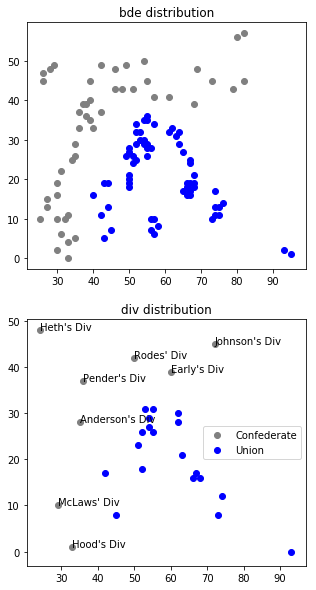
\includegraphics[width=\linewidth]{gettysburg-model.png}
    \caption{旅/师级单位位置坐标}
  \end{subfigure}
  \caption{真实情况和模型使用的数据的比较}
  \label{fig:gettysburg}
\end{figure}

In Figure~\ref{fig:gettysburgTwo} the forward probability model is illustrated and a sample of the model and observed
ally unit.

图~\ref{fig:gettysburgTwo}展示了给定两军位置时正向生成模型给出的战役发生概率密度。

\begin{figure}[ht]
  \begin{subfigure}[b]{0.49\linewidth}
    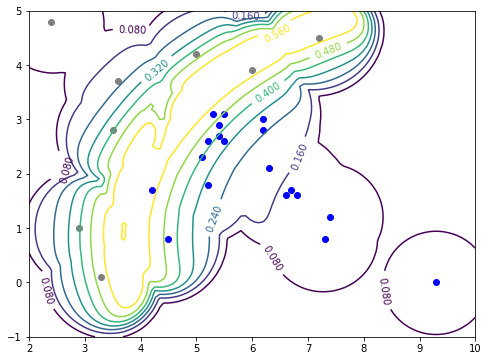
\includegraphics[width=\linewidth]{gettysburg-forward.png}
    \caption{未标准化的战役发生概率}
  \end{subfigure}
  \begin{subfigure}[b]{0.49\linewidth}
    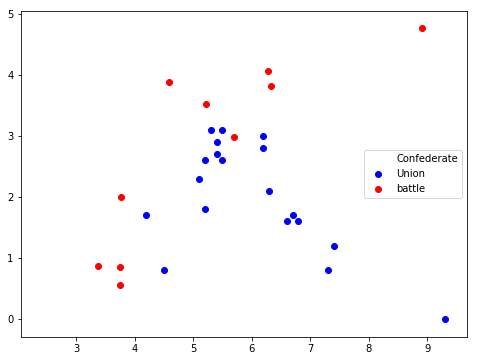
\includegraphics[width=\linewidth]{gettysburg-sample.png}
    \caption{一次采样结果+友军位置构成的模型所用数据}
  \end{subfigure}
  \caption{正向生成模型与一次采样结果}
  \label{fig:gettysburgTwo}
\end{figure}

We can run procedure described above with randomized initialized point. 
Figure~\ref{fig:gettysburgInit} show the exist-probability and converge process.

这里仍采用随机初始化验证算法有效性,随机初始点设在左上角,若算法正常运行应该收敛到与真实点接近
的位置上。迭代过程和每个阶段的存在概率密度可见于图~\ref{fig:gettysburgInit}。

\begin{figure}[ht]
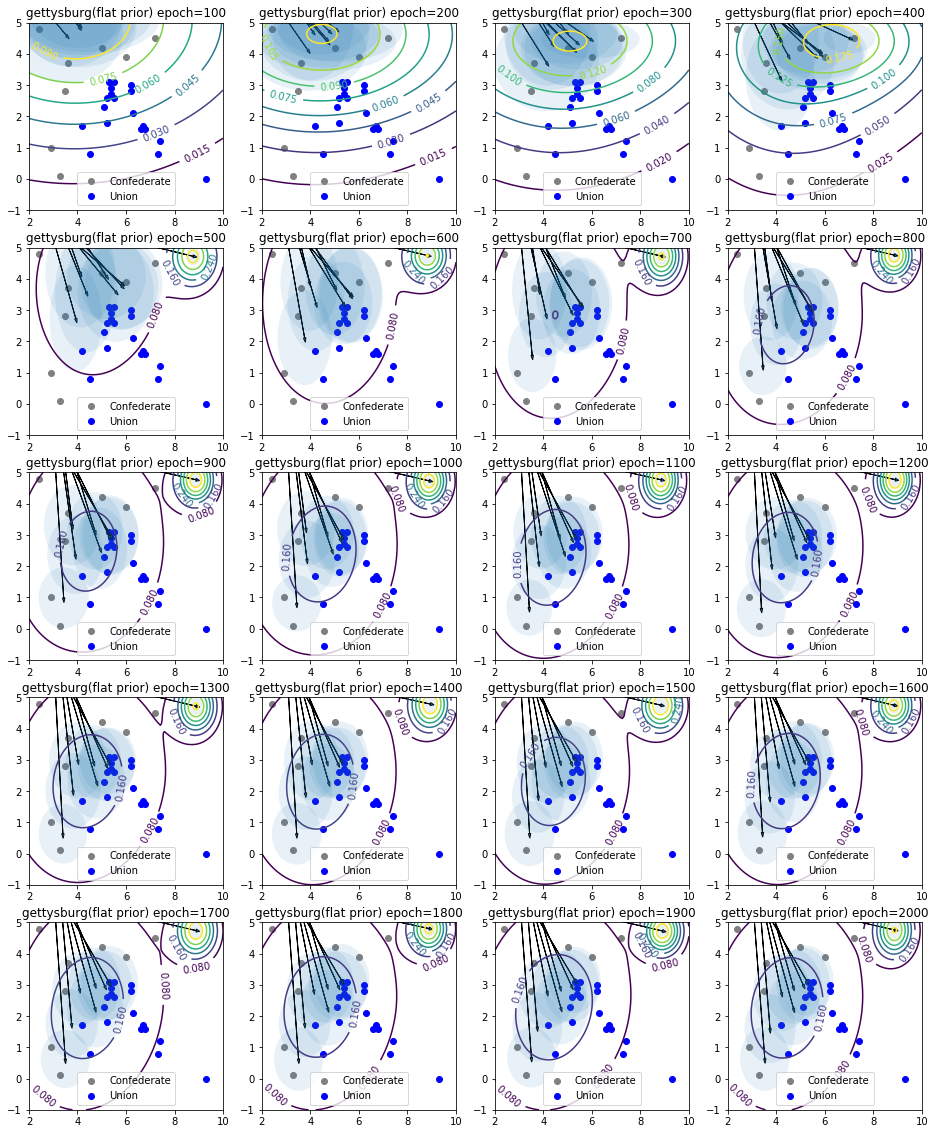
\includegraphics[width=0.99\linewidth]{gettysburg-init.png}
\caption{Iteration process for randomized initialized setting with flat prior in Gettysburg sample
均匀先验+随机初始化变分推断在葛底斯堡数据上的迭代过程}
\label{fig:gettysburgInit}
\end{figure}

It looks good, thougn the enemy units seems too close to ally. It can be solved a bit by prior.

拟合结果看上去还行,尽管敌军单位比起真实位置有点过于接近友方单位了,这个可以通过加先验惩罚解决。


\section{Extention: Size effect 扩展:规模相关模型}

The above content assurms battles and units are homogeneous. It may make sense,
but if battle and unit can include number and size information, the result will be more useful.

To extend our model to embrace the change, we can merely define the high weight the unit have,
the long radius in distance factor and large weight in estimation on center of class unit cause.

Following content use the strength of Table~\ref{tab:Confederate} and \ref{tab:Union} as weight.
The $\mu,\sigma$ used by naive bayes classifer is computed by weithted version now.
And the distance will be adujusted to $dist_{ij} = dist_{ij} \frac{\beta}{stre_i}$, the $\beta$
is seted to $6000$. So all of units of Union will be penalized, 
and a few of Confederate will be bonused for distance factor.

The Figure~\ref{fig:gettysburgInitTwo} show the result, it very like the result fited without size effect. 
It turn out that the model is steady for suct effect.

前面的部分都假定战役和单位是同质的。但是上面的葛底斯堡战役例子明显违反了这个假设,
若能整合单位的规模(战斗力,影响范围)进入模型,拟合结果应该会更好。

假定单位拥有越高的权重,则它的等效距离更短,同时在中心估计中的权重更大。

权重就使用表~\ref{tab:Confederate}与表~\ref{tab:Union}中的人数作为权重。贝叶斯分类器所用的
$\mu,\sigma$转而以加权方式计算。而距离则计算调整过的等效距离替代之前的距离,有:
$dist_{ij} = dist_{ij} \frac{\beta}{stre_i}$,其中参数$\beta$在此设为$6000$。这意味着所有的
联邦单位在距离影响上被惩罚了而一部分南方邦联单位在等效距离上得到了加成。

图~\ref{fig:gettysburgInitTwo}显示了拟合结果。它类似于没有考虑规模效应的模型的拟合结果。
这可能是因为本例中各单位规模差距并没有大到产生显著影响的程度。另外这个设定本身也有一致性问题,
考虑几个处在同一格的单位似乎应该与一个有人数为它们之和的单位落在那的效果一致,但本模型设定下
只有在中心估计上一致,等效距离上却是不一致的,这个问题在联邦军左上角师级单位密集布防的区域
显得很明显。

\begin{figure}[ht]
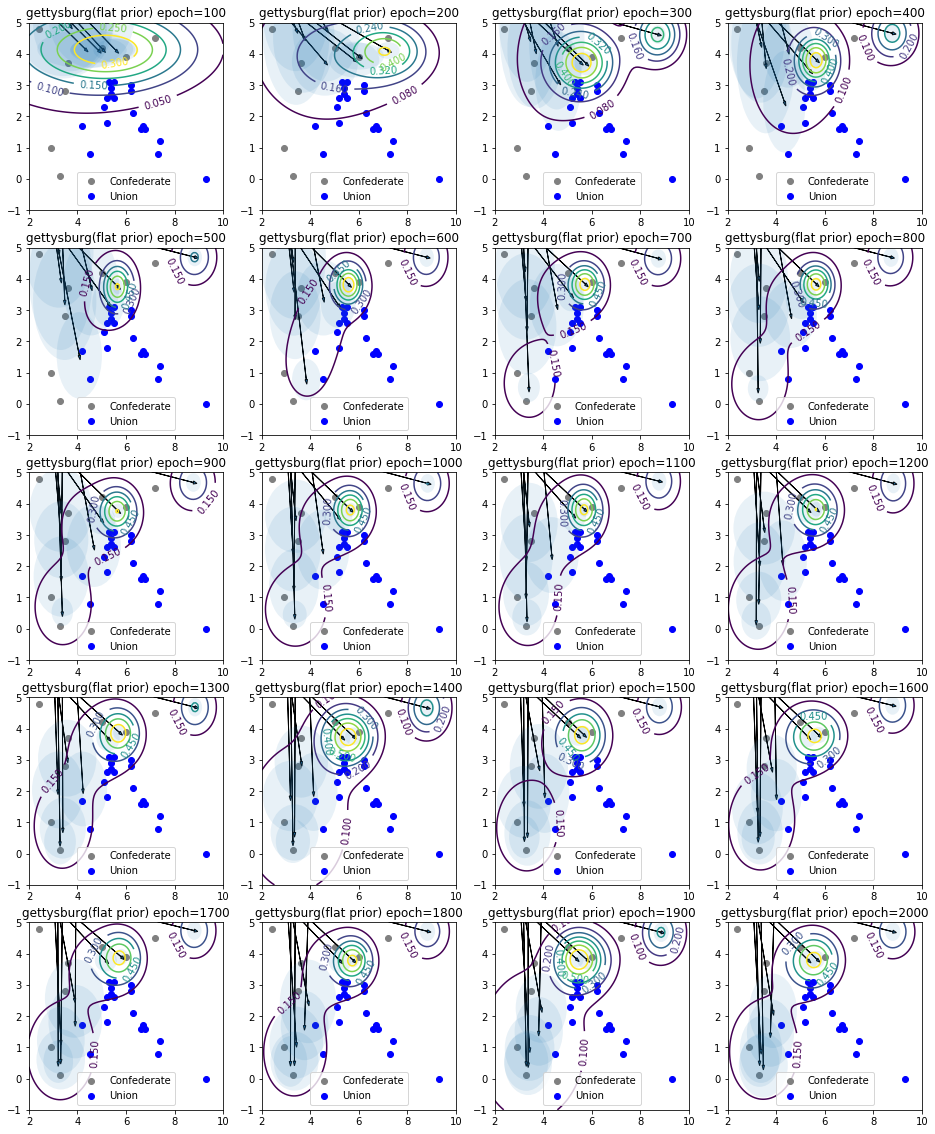
\includegraphics[width=0.99\linewidth]{gettysburg-init2.png}
\caption{Iteration process for randomized initialized setting with flat prior with Size effect
规模效应+随机初始化+均匀先验的迭代过程}
\label{fig:gettysburgInitTwo}
\end{figure}


\section{Conclusion 结论}

We present a standard bayes inference framework 
\footnote{In fact, the content of the paper have been implmented as examples of a open-source library
hosted in GitHub, see: \url{https://github.com/yiyuezhuo/bayes-torch} where yiyuezhuo is the nickname of
the writer Yueyi Zhuo} 
in a classes of prolbem in which 
two class of point(ally and enemy) will generate another class of points(battle), 
when one class is hidden(enemy).

The forward model can transformed easily to backward model to do inference due to our framework.
The inference include point detection, movement dectection with prior or adujusted prior.
They're be checked its steady and converge performance by true initialization and random initialization.
A case study about battle of Gettysburg summary the content covered by the paper. 
I wish the result can be producation environment and my game desigmning.

Desigmning the forward model, doing its inference and balancing effciency and correctness 
are interesting challenge, but useful.

本文作者基于pytorch实现了一个贝叶斯推断框架bayes-torch并用它进行了相关实验推断。
推断主要包括敌人位置,运动轨迹,存在密度的推断,分别在均匀先验和问题特定先验,真实位置初始化,
多值插值初始化,多值随机初始化的情况下验证了算法的效果。并可以运用到相关侦测问题上。

写作本文的本来目的就是为作者准备设计的一个信息屏蔽为特点的游戏做准备,不过从实际效果来看
迭代速度过慢,老要钦定参数和分类器不能自适应(Edward的贝叶斯化神经网络看上去效果不错,
不过怎么看都只会更慢而且难以解释,本文没有使用它)都是一个问题。

\section{Core code implementing the model 实现模型的主要代码}

This code section contain only the component defining the baseline model and do inference. 
The full code about figure outputing, parameter tuning and model variants code can be checked in 
\footnote{\url{https://github.com/yiyuezhuo/Undergraduate-thesis/tree/master/notebook}}.

这里列举的代码仅包括最重要的那些,样板代码和琐碎的绘图与工作函数可见于
\footnote{\url{https://github.com/yiyuezhuo/Undergraduate-thesis/tree/master/notebook}}。

%Anyway, the section is added to deal with foolish paper Duplicate check system, so you would not 
%expect its completeness since actually the source code is giant.

The top code on baseline model:

基线模型的最顶层定义代码(底层就是那些pytorch代码,忽略)

\begin{python}

# model
friend = Data(friend_point)
battle = Data(battle_point)
enemy = Parameter(enemy_point) # set real value as init value, though maybe a randomed init is more proper

logPC = Data(_logPC)

conflict_threshold = 0.2
distance_threshold = 1.0
tense = 10.0
alpha = 5.0
prior_threshold = 5.0
prior_tense = 5.0

def target():
    friend_enemy = torch.cat((friend, enemy),0)
    distance = cdist(battle, friend_enemy).min(dim=1)[0]
    

    mu = Variable(torch.zeros(2,2)) 
    sd = Variable(torch.zeros(2,2))
    
    mu[0,:] = friend.mean(dim=0)
    mu[1,:] = enemy.mean(dim=0)
    sd[0,:] = friend.std(dim=0)
    sd[1,:] = enemy.std(dim=0)
    
    conflict = torch.exp(norm_naive_bayes_predict(battle, mu, sd, logPC)).prod(dim=1)
    p = soft_cut_ge(conflict,conflict_threshold, tense = tense) * soft_cut_le(distance, distance_threshold, tense = tense)
    
    target= torch.sum(torch.log(p))
    return target

def target2():
    target1 = target()
    # location prior
    target2 = target1 + torch.sum(enemy.sum(dim=1))
    return target2

\end{python}

The movement detecting model variant:

移动监测模型变体:

\begin{python}
def target():
    target = Variable(torch.zeros(1))
    for i in range(battle_point.shape[0]):
        t = timestamp[i]
        friend = friend0*(1-t) + friend1*t
        enemy = enemy0*(1-t) + enemy1*t
        single_battle = torch.unsqueeze(battle[i],0) 
        
        friend_enemy = torch.cat((friend, enemy), 0)
        distance = cdist(single_battle, friend_enemy).min(dim=1)[0]
        
        mu = Variable(torch.zeros(2,2)) 
        sd = Variable(torch.zeros(2,2))

        mu[0,:] = friend.mean(dim=0)
        mu[1,:] = enemy.mean(dim=0)
        sd[0,:] = friend.std(dim=0)
        sd[1,:] = enemy.std(dim=0)

        conflict = torch.exp(norm_naive_bayes_predict(single_battle, mu, sd, logPC)).prod(dim=1)
        p = soft_cut_ge(conflict,conflict_threshold, tense = tense) * soft_cut_le(distance, distance_threshold, tense = tense)

        target+= torch.sum(torch.log(p))
    return target

\end{python}

The weighted model variant about forward and backward:

加权模型变体:

\begin{python}
# model for forward
reset()

friend = Data(friend_point)
battle = Data(xy)
enemy = Parameter(enemy_point) # set real value as init value, though maybe a randomed init is more proper

enemy_weight = Data(Confederate_weight)
friend_weight = Data(Union_weight)
enemy_dist_factor = Data(Confederate_dist_factor)
friend_dist_factor = Data(Union_dist_factor)


logPC = Data(_logPC)

conflict_threshold = 0.2
distance_threshold = 1.0
tense = 10.0
alpha = 5.0
prior_threshold = 5.0
prior_tense = 5.0

def target_p():
    friend_enemy = torch.cat((friend, enemy),0)
    friend_enemy_dist_factor = torch.cat((friend_dist_factor,enemy_dist_factor),0)
    
    distance = (cdist(battle, friend_enemy)*friend_enemy_dist_factor).min(dim=1)[0]
    #distance = distance * friend_enemy_dist_factor

    mu = Variable(torch.zeros(2,2)) 
    sd = Variable(torch.zeros(2,2))
    '''
    mu[0,:] = friend.mean(dim=0)
    mu[1,:] = enemy.mean(dim=0)
    sd[0,:] = friend.std(dim=0)
    sd[1,:] = enemy.std(dim=0)
    '''
    _friend_weight = torch.unsqueeze(friend_weight,1)
    _enemy_weight  = torch.unsqueeze(enemy_weight, 1)
    
    mu[0,:] = torch.sum(friend * _friend_weight,dim=0)
    mu[1,:] = torch.sum(enemy  * _enemy_weight, dim=0)
    sd[0,:] = torch.sqrt(torch.sum((friend - mu[0,:])**2 * _friend_weight, dim=0))
    sd[1,:] = torch.sqrt(torch.sum((enemy  - mu[1,:])**2 * _enemy_weight, dim=0))
    
    conflict = torch.exp(norm_naive_bayes_predict(battle, mu, sd, logPC)).prod(dim=1)
    p = soft_cut_ge(conflict,conflict_threshold, tense = tense) * soft_cut_le(distance, distance_threshold, tense = tense)
    return p

def target():
    p = target_p()
    
    target= torch.sum(torch.log(p))
    return target
    
# model for backward
reset()

friend = Data(friend_point)
battle = Data(battle_point)
enemy = Parameter(enemy_point) # set real value as init value, though maybe a randomed init is more proper

logPC = Data(_logPC)

conflict_threshold = 0.2
distance_threshold = 1.0
tense = 10.0
alpha = 5.0
prior_threshold = 5.0
prior_tense = 5.0


\end{python}

There're bayes-torch related code.

Class Model, defining the methods to do point estimation, vb and sampling.

这里列举bayes-torch代码,Model类中包含本文中使用的三种推断算法的实现

\begin{python}

class Model:
    def __init__(self):
        self.parameters = []
        self.n_parameters = 0
        self.size_parameters = []
    def reset(self):
        self.parameters = []
        self.n_parameters = 0
        self.size_parameters = []
    def add_parameter(self, variable):
        self.parameters.append(variable)
        self.n_parameters += np.prod(variable.size())
        self.size_parameters.append(variable.size())
    def set_parameter_meanfield(self, mu, omega):
        n_parameters = self.n_parameters
        param_samples_eta = np.random.normal(size=n_parameters)
        param_samples = param_samples_eta*np.exp(omega) + mu
        self.set_parameter(param_samples)
        return param_samples_eta
    def set_parameter(self, values, is_float = True):
        # values is a flatten numpy array
        start = 0
        for param in self.parameters:
            param_size = np.prod(param.size())
            section = values[start:start+param_size].reshape(param.size())
            tensor = torch.from_numpy(section)
            if is_float:
                tensor = tensor.float()
            param.data = tensor
            start += param_size
    def collect_parameter_grad(self):
        grad = np.empty(self.n_parameters)
        start = 0
        for param in self.parameters:
            param_size = np.prod(param.size())
            grad[start:start+param_size] = param.grad.data.numpy().copy().ravel()
            start += param_size
        return grad
    def collect_parameter(self):
        res = np.empty(self.n_parameters)
        start = 0
        for param in self.parameters:
            param_size = np.prod(param.size())
            res[start:start+param_size] = param.data.numpy().copy().ravel()
            start += param_size
        return res
    def grad_q_meanfield(self, target_f, mu, omega, q_size=10, lr = 0.01):
        n_parameters = self.n_parameters
        
        mu_grad = np.zeros(n_parameters)
        omega_grad = np.zeros(n_parameters)
        
        optimizer = torch.optim.SGD(self.parameters, lr=lr)
        # optimizer only serve to zero_grad.
        
        for i in range(q_size):
            
            param_samples_eta = self.set_parameter_meanfield(mu, omega)
            
            optimizer.zero_grad()
            target = target_f()
            target.backward()
            
            param_grad = self.collect_parameter_grad()
            mu_grad += param_grad
            omega_grad += param_grad * param_samples_eta
        
        mu_grad /= q_size
        omega_grad /= q_size
        omega_grad *= np.exp(omega)
        omega_grad += 1.0
        
        return mu_grad,omega_grad
            
    def vb_meanfield(self, target_f, mu=None,omega=None, zero_init=False, 
                     n_epoch = 100, lr=0.01, q_size = 10):
        n_parameters = self.n_parameters
        
        if mu is None:
            if zero_init:
                mu = np.zeros(n_parameters)
            else:
                mu = np.array(self.collect_parameter())
        if omega is None:
            omega = np.zeros(n_parameters) # sigma=exp(omega) = 1
        
        #optimizer = torch.optim.SGD(self.parameters, lr=lr)
        
        for i in range(n_epoch):
            mu_grad,omega_grad = self.grad_q_meanfield(target_f, mu, omega, q_size = q_size)
            mu += lr * mu_grad
            omega += lr * omega_grad
        
        return mu,omega
        
        
    def vb_fullrank(self, target_f):
        raise NotImplementedError
    def vb_meanfield_format(self, res):
        # res = (mu, omega) -> {Parameter1: {'mu': mu1, 'sigma': exp(omega1)}...}
        mu, omega = res
        
        return_dict = {}
        start = 0
        for param in self.parameters:
            param_size = np.prod(param.size())
            _mu = mu[start:start+param_size].reshape(param.size())
            _omega = omega[start:start+param_size].reshape(param.size())
            return_dict[param] = {'mu':_mu,'omega':_omega}
            start += param_size
        return return_dict

    def vb(self, target_f, method = 'meanfield', format=False, 
                 reload=False, **kwargs):
        if method == 'meanfield':
            res = self.vb_meanfield(target_f, **kwargs)
            if not format:
                return res
            self.set_parameter(res[0])
            grad = self.grad(target_f) 
            grad_size = np.sum(grad**2)
            converge = grad_size < 0.01
            report = dict( method = 'meanfiled', 
                           est = self.vb_meanfield_format(res),
                           grad = grad,
                           grad_size = grad_size,
                           converge = converge)
            if reload:
                self.set_parameter(res[0])
            return report
        if method == 'fullrank':
            return self.vb_fullrank(target_f, **kwargs)
        raise NotImplementedError
    def sampling_hmc(self, target_f, epsilon=0.01, L=20, M=100):
        
        def grad(theta):
            self.set_parameter(theta)
            return self.grad(target_f)
        def likelihood(theta):
            self.set_parameter(theta)
            return target_f().data.numpy()
        
        sample =[]
        sample.append(self.collect_parameter())
        accept_list = []
        
        for m in range(M):
            r0 = np.random.normal(size=self.n_parameters)
            r = r0
            theta0 = sample[-1]
            theta = theta0.copy()
            
            for i in range(L):
                r = r + 0.5 * epsilon * grad(theta)
                theta = theta + epsilon * r
                self.set_parameter(theta)
                r = r + 0.5 * epsilon * grad(theta)
            odd_up = np.exp(likelihood(theta)-0.5*np.dot(r,r))
            odd_bottom = np.exp(likelihood(theta0)-0.5*np.dot(r0,r0))
            alpha = min(1,odd_up/odd_bottom)
            accept_list.append(alpha)
            
            if np.random.random() < alpha:
                sample.append(theta)
            else:
                sample.append(theta0)
        return sample
        

    def sampling(self, target_f, method= 'hmc', **kwargs):
        #trace = []
        #raise NotImplementedError
        if method == 'hmc':
            return self.sampling_hmc(target_f, **kwargs)
        if method == 'nuts':
            return self.sampling_nuts(target_f, **kwargs)
        raise NotImplementedError
    def optimizing(self, target_f, lr=0.01, n_epoch = 1000):
        '''
        After optimizing run, the result is stored in original torch variable.
        target_f don't have any parameter, since the class serve to delete the trouble
        '''
        optimizer = torch.optim.SGD(self.parameters, lr=lr)
        
        for epoch in range(n_epoch):
            optimizer.zero_grad()
            target = target_f()
            loss = -target
            loss.backward()
            optimizer.step()
    def grad(self, target_f):
        fake_lr = 1.0
        optimizer = torch.optim.SGD(self.parameters, lr=fake_lr)
        optimizer.zero_grad()
        target = target_f()
        target.backward()
        return self.collect_parameter_grad()

\end{python}

Other helper function in bayes-torch:

最相关的bayes-torch其他函数:

\begin{python}
def torch_norm_log_prob(X,mu,sd):    
    temp = -(X - mu)**2/(2*sd) 
    temp = temp - 0.5 * torch.log(2.0 * np.pi * sd)
    return temp

def torch_norm_naive_bayes_predict(X,mu,sd,logPC):
    # X: sample_size * features
    # mu: class_size * features
    # sd: class_size * featrues
    # log_PC class_size
    n_class = logPC.size()[0]
    n_feature = X.size()[1]
    n_sample = X.size()[0]
    _X = torch_tile(X,[1,n_class]).resize(n_sample,n_class,n_feature)
    cp = torch_norm_log_prob(_X, mu, sd).sum(dim=2) + logPC  
    log_predict_prob = torch_transpose((torch_transpose(cp) - torch_logsumexp(cp,dim=1)))
    return log_predict_prob
    
def torch_logsumexp(X,dim=0):
    # numpy have this function
    return torch.log(torch.exp(X).sum(dim=dim))

def torch_tile(X,repeats):
    # torch.repeat ~ numpy.tile
    return X.repeat(*repeats)


def torch_soft_cut_ge(x,threshold,tense=1.0):
    return torch.sigmoid(tense*(x-threshold))

def torch_soft_cut_le(x,threshold,tense=1.0):
    return torch.sigmoid(tense*(-x+threshold))


\end{python}

Notebook specific code, the density estimation:

Jupyter notebook实验中主要绘图和密度估计代码:

\begin{python}

def prob_point(x,y,dx,dy,_mu,_omega):
    mu = _mu.reshape(enemy_point.shape)
    sigma = np.exp(_omega.reshape(enemy_point.shape))
    x = np.reshape(x,(-1,1))
    y = np.reshape(y,(-1,1))
    px  = stats.norm.cdf((x-mu[:,0])/sigma[:,0])
    pdx = stats.norm.cdf((x+dx-mu[:,0])/sigma[:,0])
    py  = stats.norm.cdf((y-mu[:,1])/sigma[:,1])
    pdy = stats.norm.cdf((y+dy-mu[:,1])/sigma[:,1])
    return (pdx - px) * (pdy - py)

def prob_exist(x,y,dx,dy,_mu,_omega):
    ememy_prob = prob_point(x,y,dx,dy,_mu,_omega)
    return 1-np.prod((1 - ememy_prob).T,axis=0) 

def prob_exist_limit(x,y,_mu,_omega,step=0.1):
    p = prob_exist(x-step,y-step,2*step,2*step,_mu,_omega)
    return p/(4*step*step)

def show_change(show=False):
    display_data()
    for i in range(enemy_point.shape[0]):
        #s = 0.1
        plt.arrow(enemy_point[i][0], enemy_point[i][1], enemy.data[i][0] - enemy_point[i][0], enemy.data[i][1] - enemy_point[i][1],head_width=0.1)
    plt.legend()
    if show:
        plt.show()


def show_ellipse(mu,sd):
    from matplotlib.patches import Ellipse
    
    #ax = plt.subplot(111)
    ax = plt.gca() # get current axe, the lame method to support command style
    show_change(show=False)
    #res_reshaped = [r.reshape(enemy_point.shape) for r in res]
    for i in range(enemy_point.shape[0]):
        mu_x,mu_y = mu[i]
        sd_x,sd_y = sd[i]
        e=Ellipse((mu_x,mu_y), sd_x, sd_y, 0)
        e.set_clip_box(ax.bbox)
        e.set_alpha(0.1)
        ax.add_artist(e)
        
    #plt.show()
    
    
def show_vb(vb_res):
    res = vb_res
    model.set_parameter(res[0])
    res_reshaped = [r.reshape(enemy_point.shape) for r in res]
    mu = res_reshaped[0]
    sd = np.exp(res_reshaped[1])
    show_ellipse(mu,sd)
    
def multi_enemy_setting_show_exist_density(_enemy_point, target, title_string):
    reset_enemy(_enemy_point)
    res = vb(target)
    show_vb(res)
    p_exist = prob_exist_limit(xy[:,0],xy[:,1],res[0],res[1],step=0.001).reshape(xx.shape)
    CS = plt.contour(xx,yy,p_exist)
    #plt.contour(xx, yy, p_exist)
    plt.clabel(CS)
    #plt.title(title_string.format(i))
    plt.gca().set_title(title_string.format(i))
    plt.legend()

    
    
plt.figure(figsize=(16,20)) #(x,y)
for i in range(2, 10):
    interp_x = np.linspace(_enemy_point[:,0].min(),_enemy_point[:,0].max(),i)
    interp_y = np.interp(interp_x, _enemy_point[:,0], _enemy_point[:,1])
    interp_xy = np.c_[interp_x,interp_y]
    plt.subplot(4, 4, i-1)
    multi_enemy_setting_show_exist_density(interp_xy, target , '{} with flat prior')

for i in range(2, 10):
    interp_x = np.linspace(_enemy_point[:,0].min(),_enemy_point[:,0].max(),i)
    interp_y = np.interp(interp_x, _enemy_point[:,0], _enemy_point[:,1])
    interp_xy = np.c_[interp_x,interp_y]
    plt.subplot(4, 4, 8+i-1)
    multi_enemy_setting_show_exist_density(interp_xy, target2 , '{} with diag prior')

    #multi_enemy_setting_show(interp_xy, target2, '{} with diag prior')
plt.title('multiple number setting for vb with exist density')
plt.show()


\end{python}



%\begin{python}
%\end{python}

\bibliography{paper} 
\bibliographystyle{ieeetr}

\end{document}